\documentclass[withoutpreface,bwprint]{cumcmthesis} %去掉封面与编号页
\usepackage{graphicx}
\title{论文题目}
\tihao{B}            % 题号
\baominghao{4321}    % 报名号
\schoolname{你的大学}
\membera{成员A}
\memberb{成员B}
\memberc{成员C}
\supervisor{指导老师}
\yearinput{2017}     % 年
\monthinput{08}      % 月
\dayinput{22}        % 日

\begin{document}
\begin{abstract}
    本文研究了在不同类型的待测海域内的多波束测深的覆盖宽度及相邻条带之间重叠率,
    在二维平面内,构建了在固定坡度下关于覆盖宽度及相邻条带之间重叠率的多波束测线二维平面模型;
    在三维空间中,确定了多波束测线三维立体模型并提出了三维多波束测线的优化指标及任意海域中多波束测线的设计方法;
    

    \begin{enumerate}
        \item \textbf{针对问题一}:首先,根据平坦海域多波束测深的工作原理,推导出覆盖宽度 $W$ 和重叠率 $\eta$ 的计算公式。并再次基础上定义了一般情况的重叠了的
        定义:每个覆盖宽度 $W$ 的重叠宽度 $W_\text{重}$ 与覆盖宽度总和的比值。
        ,针对坡度为 $\alpha$ 的二维海底斜面的情况,分以侧线为轴线的左侧宽度 $W_1$ 和右侧宽度 $W_2$这两部分,分开讨论。
        结合几何推理得出的关系式以及\textbf{正弦定理},建立左侧宽度 $W_1$ 和右侧宽度 $W_2$ 与海底斜面坡度 $\alpha$ 的关系,进而得出总覆盖宽度;
        然后,分析相邻条带重叠率的计算公式,建立相邻条带重叠率与总覆盖宽度之间的关系。
        最后,综合以上分析,建立多波束测线二维平面模型。
        在题目给出参数情况下,对覆盖宽度及重叠率进行遍历求解
        得出结果。
        \item \textbf{针对问题二}:为了解决测绘具有固定坡度的三维地形图,定义了三维空间中的覆盖宽度,为了简化问题,引入\textbf{矢量分解}的方法
        分别研究了以$X$轴和$Y$轴方向的位移分量对覆盖宽度在$X$轴和$Y$轴方向的影响。最后利用矢量合成公式得出总覆盖宽度公式,建立多波束测线三维立体模型。
        %  \begin{table}[htbp]
        %     \caption{问题二的计算结果}
        %     \centering
        %     \begin{tabular}{cc|cccccccc}
        %         \toprule[2pt]
        %         \multirow{2}{*}{覆盖宽度/m} & \multicolumn{8}{c}{测量船距海域中心点处的距离/海里}  \\
        %         \cmidrule(lr){3-10}
        %         & & 0 & 0.3 & 0.6 & 0.9 & 1.2 & 1.5 & 1.8 & 2.1 \\
        %         \midrule[1pt]
        %         & 0 & 415.7 & 466.1 & 516.5 & 566.9 & 617.3 & 667.7 & 718.1 & 768.5 \\
        %         & 45 & 416.2 & 451.9 & 487.5 & 523.2 & 558.9 & 594.6 & 630.2 & 665.9 \\
        %         测线 & 90 & 416.7 & 416.7 & 416.7 & 416.7 & 416.7 & 416.7 & 416.7 & 416.7 \\
        %         方向 & 135 & 416.2 & 380.5 & 344.8 & 309.2 & 273.5 & 237.8 & 202.1 & 166.5 \\
        %         夹角 /$^\circ$  & 180 & 415.7 & 365.3 & 314.9 & 264.5 & 214.1 & 163.7 & 113.3 & 62.9\\
                
        %         \bottomrule[2pt]
        %     \end{tabular}
        % \end{table}
        \item \textbf{针对问题三}:在问题二的基础上,推导并设立了多波束测线的三维优化指标\textbf{单位距离扫描增益}以及三维相邻条带重叠率,
        接着基于问题二的思想继续对位移矢量进行正交分解。据此建立了多波束测线单目标优化问题,为了降低计算复杂度,
        将建立起的单目标优化问题分解为两个子问题得出最优测线方向,我们有结果对于驶向浅水区方向以平行于等高线方向航行即$
        \beta=90^{\circ} \mathrm{C}$ 通过\textbf{微元法},对子问题进行求解对于驶向深水区方向以垂直于等高线方向航行即$\beta=0^{\circ} \mathrm{C}$ 
        以及 最短测线长度127990$m$。
        
        
        
        
        
        \item \textbf{针对问题四}:为了得到在一般矩形待测海域的多波束测线设计模型,利用\textbf{微元法}将一般矩形
        待测海域离散化为若干个平面小矩形,并以中心的海水深度近似整个平面矩形深度。根据题目给出的条件,设计设计指标,设计了最优测线轨迹,其结果如下表:
        
        \begin{table}[!htbp]
        \caption{问题四的计算结果} 
        \centering
        \begin{tabular}{ccc}
            \toprule[2pt]
            测线总长度/m & 漏测海区占总待测海域面积的百分比 & 重叠率超过20\%的测线总长度 \\
            \midrule[1pt]
            441183.44 & 0.06837 & 3000.24\\
            \bottomrule[2pt]
        \end{tabular}
    \end{table}
     
    \end{enumerate}
    \keywords{多波束探测系统\quad  单目标优化\quad   矢量合成与分解\quad 微元法}
\end{abstract}

    \section{问题重述}
    \subsection{问题背景}
    多波束测深技术在海洋深度测量中具有广泛的应用, 其实际工作方式如图~\ref{30}~所示,但其覆盖宽度 $W$ 受到换能器开角 $\theta$ 和水深 $D$ 的影响,从而导致相邻测线之间的重叠率 $\eta$ 不稳定。
    为确保数据的完整性和测量质量,通常要求相邻条带之间具有一定的重叠率,然而,海底地形的复杂起伏使得传统的基于平均水深或最浅水深的测线间隔设计存在问题。
    使用平均水深设计可能导致在水深较浅处出现漏测,而使用最浅水深设计则可能导致在水深较深处产生过多的数据重叠,从而影响测量效率。
    因此,需要寻找一种优化的测线间隔设计方法,以适应不同海底地形条件下的多波束测深需求,提高测量的准确性和效率。

    \begin{figure}[htbp]
        \centering
        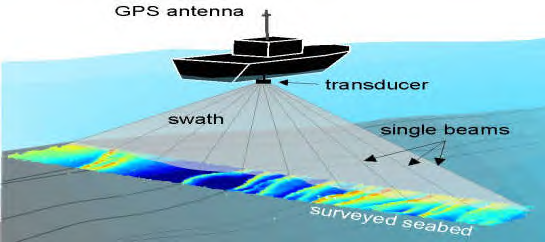
\includegraphics[height=0.25\textheight]{问题背景.png}
        \caption{多波束测深示意图}
        \label{30}
    \end{figure}

    \subsection{问题重述}
    \begin{enumerate}
    \item \textbf{问题一}:对于二维平面内坡度为$\alpha$的海域进行多波束探测,目标是建立数学模型,确定扫描宽度覆盖$W$和相邻扫描带之间的重叠率$\eta$。
    \item \textbf{问题二}:考虑一个三维坡度为$\alpha$的待测矩形区域,其中测量方向与海底坡度法线在水平平面上的投影之间的角度记为$\beta$。目标是建立数学模型,确定三维固定坡度多波束测深的扫描宽度覆宽度$\eta$。
    \item \textbf{问题三}:在一个南北方向长$2$海里、东西方向宽$4$海里、坡度$\alpha$为$1.5°$的矩形海域内,其中心海水深度为$110m$,多波束换能器的开角为$120°$。难点在于设计一组最短的测量线,以确保完全覆盖整个测量海域。此外,相邻扫描带之间的重叠率应满足$10\%$到$20\%$的要求。
    \item \textbf{问题四}:题目给出一组若干年前在南北方向长5海里、东西方向宽4海里的海域中使用单波束深度测量获得的海水深度测量数据,目标是利用这组数据来协助规划多波束测深船的测量线路。
    
    测线的设计须符合以下要求:
    \textbf{1.} 在每个扫描带内最大程度地覆盖整个测量海域;
    \textbf{2.} 确保相邻扫描带之间的重叠率尽量低于20\%;
    \textbf{3.} 最小化测线的总长度。
    
    设计具体测线后须计算以下指标:
    \textbf{1.} 测线的总长度;
    \textbf{2.} 未测区域在总测量海域面积中所占的百分比;
    \textbf{3.} 在重叠区域内超过20\%重叠的总长度。
    \end{enumerate}
    
    \section{问题分析}
    \begin{itemize}
        \item \textbf{针对问题一}:目标是建立在坡度为$\alpha$的海底斜面上的多波束测线二维平面模型,关注指标为多波束覆盖宽度与相邻条带重叠率;
        首先,根据平坦海底情况下多波束测深的工作原理,推导出覆盖宽度 $w$ 和重叠率 $\eta$ 的计算公式。
        接着,针对坡度为 $\alpha$ 的海底斜面的情况,分以侧线为轴线的左侧宽度 $W_1$ 和右侧宽度 $W_2$这两部分,分开讨论。
        结合几何推理以及\textbf{正弦定理}得出的关系式,建立左侧宽度 $W_1$ 和右侧宽度 $W_2$ 与海底斜面坡度 $\alpha$ 的关系,进而得出总覆盖宽度;
        然后,分析平坦海底情况下相邻条带重叠率$\eta$的计算公式,建立相邻条带重叠率$\eta$与总覆盖宽度之间$W$的数学模型。
        最后,综合以上分析,建立多波束测线二维平面模型。
     
        \item \textbf{针对问题二}:目标是建立在坡度为$\alpha$的矩形待测海域上的多波束测线三维立体模型,主要关注点是三位空间中多波束覆盖宽度$W$。
        不同于二维空间中覆盖宽度变化的自由度仅存在一维,在三维空间中,覆盖宽度的变化的自由度存在两个两个维度,增加了旋转角$\beta$。
        因此在本题中,引入了\textbf{矢量分解}的方法,将覆盖宽度正交分解,以减小其变化自由度的维度,从而简化问题。
        首先,利用海底坡面的法向在水平面上的投影为 $X$ 轴建立空间直角坐标系,
        第二,根据\textbf{矢量分解}的原理,再将沿测线方向每点测量的覆盖宽度和相对于起始点的位移分别沿 $X$ 轴方向和 $Y$ 轴方向进行分解;
        其次,分别推导分解后的$X$方向位移,$Y$方向位移对测线覆盖宽度$X$方向分量$Y$方向分量的影响,
        最后,通过\textbf{矢量合成}得出总覆盖宽度公式,建立多波束测线三维立体模型。
        \item \textbf{针对问题三}:目标是建立在坡度为$\alpha$的矩形待测海域上的多波束测线三维优化模型,优化目标为在完全覆盖整个待测海域且满足测线间重叠率$10\%$到$20\%$的前提下,最小化测线的总长度。
        首先,根据问题二建立多波束测线三维立体模型,进一步推导得到多波束测线的三维优化指标\textbf{单位距离扫描增益}$S_x(x)$和三维相邻条带重叠率$\eta_{\text{三维}}$;
        第二,根据提出的优化指标建立多波束测线\textbf{三维单目标优化模型};
        其次,将建立的单目标问题分解为方向角$\beta$优化和测线数量优化两个子问题;
        最后,通过\textbf{微元法}对子问题进行求解,得出最优方向角$\beta$和最优测线数量,进而得到最优测线设计方案。
        \item \textbf{针对问题四}:目标是得到在一般矩形待测海域的多波束测线设计模型,目标为为待测海域设计尽可能满足条件的测线并计算指标。
        不同于问题二和问题三中,坡度固定的坡面,在一般海域中,其覆盖宽度由多个变量共同决定,难以计算。因此,本问中引入了\textbf{微元法},一般矩形待测海域离散化为若干个平面小矩形,以简化问题。
        首先,根据\textbf{微元法},将一般矩形待测海域离散化为若干个平面小矩形,并以中心的海水深度近似整个平面矩形深度;
        其次,根据题目给出的条件,设计设计指标,使尽量覆盖整个海域的情况下,使重叠率保持在$20\%$以下并使测线总长度近可能减小;
        最后,通过\textbf{微元法},进行逐点决策,得出最优测线设计方案。
    \end{itemize} 

    \section{模型的假设}
    \begin{assumption}
        \label{assumption1}:船只在海面上的移动被近似为在二维平面上的水平运动。
    \end{assumption}
    
    \begin{assumption}
        \label{assumption2}:忽略海底坡度的表面曲率,将其视为平坦表面。
    \end{assumption}
    
    \begin{assumption}
        \label{assumption3}:不考虑复杂海底条件导致的虚假回声。
    \end{assumption}
    
    \begin{assumption}
        \label{assumption4}:假设多波束声纳系统的测量误差可以忽略不计。
    \end{assumption}

    \section{符号说明}
    \rowcolors{2}{gray!20}{gray!10}
    \begin{longtable}{c c m{\textwidth}} % 调整第三列宽度
      \rowcolor{white}  
      \toprule[2pt] % 顶部横线
        % 表头
        符号 & 含义 \\
        \midrule[1pt] % 标题和内容之间的横线
        \endfirsthead % 第一页表头
        % 后续页面表头重复
        符号 & 含义 \\
        \midrule[1pt]
        \endhead % 结束当前表头,后续页面表头重复
        % 表格内容开始
        $W(x)$ & 沿测线方向每点探测的覆盖宽度 \\
        $S(x)$ & 多波束测线覆盖面积 \\
        $S_x(x)$ & 沿测线方向上单位距离扫描面积 \\
        $E$ & 单位距离扫描面积$S_x(x)$的增加率 \\
        $\eta_{\text{三维}}$ & 三维效率指标 \\
        $x_i$ & 优化问题中的变量 \\
        $\beta$ & 测线方向与海底坡面的法向在水平面上投影的夹角 \\
        $\alpha$ & 海底坡度 \\
        $D$ & 海域中心点处海水深度 \\
        $Z$ & 垂直于水平面方向 \\
        $X$ & 海底坡面的法向在水平面的投影 \\
        $Y$ & 坡面法向与水平面法向组成的平面法向 \\
        $D_\text{水平}$ & 沿$Y$方向的位移分量 \\
        $D_0$ & 测线起始位置时的海水深度 \\
        $W_Y$ & $Y$方向的覆盖宽度 \\
        $W_X(x)$ & $X$方向的覆盖宽度 \\
        $D(x)$ & 测线方向测量船距海域中心点处距离为$x$时的海水深度 \\
        % 表格内容结束
        \bottomrule[2pt] % 底部横线
        % % 添加表格标签以便在文中引用
        % \label{tab:symbols}
    \end{longtable}
    \rowcolors{2}{white}{white} % 跨页后续页面表格需要重新设置颜色
     
    \section{问题一模型建立与求解}
    \subsection{多波束测线二维平面模型}

    \begin{table}[H]
        \caption{Network Parameter Setting}
        \centering
        \begin{tabular}{|c|c|c|c|}
          \hline
          Parameter Symbol&Parameter Value&Parameter Symbol&Parameter Value\\
          \hline
          $P_{h}$&$1.5 \mathrm{~ W}$&$P_{f}$&$8 \mathrm{~ W}$\\
          \hline
          D&$5 $&B&$50 \mathrm{~ MHz}$\\
          \hline
          $P_{r}$&$12 \mathrm{~ dBm}$&$M$&$30 \mathrm{~ MB}$\\
          \hline
          V&$25 \mathrm{~ m/s}$&$N$&36\\
          \hline
          $\gamma$&0.99&$\aleph$&$10^{-1}$\\
          \hline
          $f_r$&$1500 \mathrm{~ cycles/bit}$&$f_e$&$1000 \mathrm{~ cycles/bit}$\\
          \hline
          $H_0$&$40 \mathrm{~ m}$&$\mu$&2\\
          \hline
          $v_1$&2&$v_2$&1\\
          \hline
        \end{tabular}
      \end{table}

      \begin{algorithm}[H]
        \caption{Intelligent UAV Planning Approach using D3QN-DDPG for Mobile IRS-assisted UAV-enabled MEC Network}
        \label{alg1}
        \begin{algorithmic}[1]
        \Require Initialize the parameters of the D3QN and DDPG networks.
        \Ensure Output the optimal UAV planning actions.
        
        \State Initialize the parameters of the D3QN networks: $\eta$, $\xi$, and $\omega$;
        \State Initialize the parameters of the DDPG networks: $\rho$ and $\upsilon$;
        \State Copy the same network parameters to target networks: $\eta^{-} \leftarrow \eta$, $\xi^{-} \leftarrow \xi$, $\omega^{-} \leftarrow \omega$, $\rho^{-} \leftarrow \rho$, and $\upsilon^{-} \leftarrow \upsilon$;
        \State Initialize the action: $a_0=\left\{q_{r,0}, q_{i,0}, \{\boldsymbol{\phi}_{i,0}\},\sigma_{e,0},\beta_{d,0}, \delta_0\right\}$;
        
        \For{each epoch}
        \State The state is obtained when the agent executes the action $a_{t-1}$, represented by $s_t=\biggl\{a_{t-1}, T_t, E_t\biggr\}$;
        \For{each time step ${t}$}
        \State The discrete action $a_{t}^1$ is obtained using the D3QN algorithm, and the continuous action $a_{t}^2$ is obtained using the DDPG algorithm, $a_{t}=\left\{a_{t}^1, a_{t}^2\right\}$;
        \State Action $a_{t}$ is executed by the agent to obtain the reward $r_{t}$ and transition to the new state $s_{t+1}$.
        \State The experience $\left\{s_{t}, a_{t}, r_{t+1}, s_{t+1}\right\}$ is built and stored in the experience buffer;
        \State Samples of size $L$ are obtained from the experience buffer;
        \State Update the actor network parameter $\delta$ and the critic network parameters $\upsilon$ in the DDPG evaluation networks;
        \State Update the parameters $\eta$, $\xi$, and $\omega$ in the D3QN networks;
        \State Update $\delta^{-}$ in the DDPG target actor network;
        \State Update $\xi^{-}$ in the target DDPG critic network;
        \EndFor
        \EndFor
        \end{algorithmic}
      \end{algorithm}


    单波束测深是利用声波在水中的传播特性来测量水体深度的技术。声波在均匀介质中作匀
速直线传播,在不同界面上产生反射,利用这一原理,从测量船换能器垂直向海底发射声波信
所示。由于单波束测深过程中采取单点连续的测量方法,因
此,其测深数据分布的特点是,沿航迹的数据十分密集,而在测线间没有数据。
    \subsubsection{平坦条件下多波束测线二维平面模型}
    \begin{figure}[htbp]
        \centering
        \begin{minipage}[b]{0.35\textwidth}
            % 左边的文字、
            多波束测深系统是在单波束测深的基础上发展起来的,
            多波束探测系统在与航迹垂直的平面内发射多个波束,其工作原理如图~\ref{1}~所示。在海底平坦的地区,其能够测量沿测线轴线具有一定宽度的全覆盖水深条带。
            其覆盖宽度可表示为 $W$,$W$ 与换能器开角 $\theta$ 和水深 $D$ 的关系,可表示为:
        
    
        \end{minipage}%
        \begin{minipage}[b]{0.4\textwidth}
            % 右边的图片
            \centering
            
\includegraphics[height=0.19\textheight]{单波平面.png}
            \caption{多波束测深工作原理}
            \label{1}
        \end{minipage}
    \end{figure}

    \begin{equation}
        W = 2 \times D \cdot \tan\left(\frac{\theta}{2}\right) \text{。}
    \end{equation}
    

    如图~\ref{1}~所示,当两个测线相互平行时,其重叠率 $\eta$ 可以表示为每个覆盖宽度 $W$ 的重叠宽度 $W_\text{重}$ 与覆盖宽度总和的比值,具体计算公式如下:
    \begin{equation}
        \eta = \frac{W_\text{重} \times 2}{W + W} \text{。}
        \label{eq2}
    \end{equation}
    其中 $W_\text{重} = 2 \cdot \left(\frac{W}{2} - d\right)$,经化简得:
    \begin{equation}
        \eta = 1 - \frac{d}{W} \text{。}
    \end{equation}
    \subsubsection{固定坡度条件下多波束测线二维平面模型}
    对于坡度为 $\alpha$ 的海底坡面,如图~\ref{3}~所示,系统的覆盖宽度 $W$ 是由以侧线为轴线的左侧宽度 $W_1$ 和右侧宽度 $W_2$。
    左侧宽度 $W_1$ 和右侧宽度 $W_2$ 的具体计算公式考虑了角度、三角函数和坡度等参数,使得模型能够准确描述不同条件下的覆盖宽度。
    
    结合题目已知条件以及几何推理,可以得出$\delta_1$、$\delta_2$和$\alpha$的三者之间的关系:
    \begin{equation}
        \left\{
        \begin{aligned}
            \delta_1 &= \alpha + \frac{\pi}{2} \\
            \delta_2 &= \frac{\pi}{2} - \alpha - \frac{\theta}{2} \\
            \delta_2 &= \frac{\pi} - \delta_1 + \frac{\theta}{2}
        \end{aligned}
        \right.
    \end{equation}

    \begin{figure}[htbp]
        \centering
        \begin{minipage}[c]{0.48\textwidth}
            \centering
            
\includegraphics[height=0.2\textheight]{单波斜面.png}
            \subcaption{}
        \end{minipage}
        \begin{minipage}[c]{0.48\textwidth}
            \centering
            
\includegraphics[height=0.2\textheight]{单波斜面标注.png}
            \subcaption{}
        \end{minipage}
        \caption{单测线斜坡中多波束探测的工作原理}
        \label{3}
    \end{figure}

    所以对于左侧宽度 $W_1$,可得出以下公式:
    \begin{equation}
        \frac{D}{\sin\left(\frac{1}{2}\pi - \alpha - \frac{1}{2}\theta\right)} = \frac{W_1}{\sin\left(\frac{1}{2}\theta\right)} \text{。}
    \end{equation}
    经化简得:
    \begin{equation}
        W_1 = \frac{D \cdot \sin\left(\frac{\theta}{2}\right)}{\cos\left(\frac{\theta}{2}+\alpha\right)} \text{。}
    \end{equation}
    同理,对于右侧宽度 $W_2$:
    \begin{equation}
        \frac{D}{\sin\left(\frac{1}{2}\pi + \alpha - \frac{1}{2}\theta\right)} = \frac{W_2}{\sin\left(\frac{1}{2}\theta\right)} \text{。}
    \end{equation}
    经化简得:
    \begin{equation}
        W_2 = \frac{D \cdot \sin\left(\frac{\theta}{2}\right)}{\cos\left(\alpha - \frac{\theta}{2}\right)} \text{。}
    \end{equation}
    因此,总覆盖宽度 $W$ 由以下公式给出:
    \begin{equation}
        W = \frac{D \cdot \sin\left(\frac{\theta}{2}\right)}{\cos\left(\alpha - \frac{\theta}{2}\right)} + \frac{D \cdot \sin\left(\frac{\theta}{2}\right)}{\cos\left(\alpha + \frac{\theta}{2}\right)} \text{。}
        \label{eq1}
    \end{equation}

    对于双测线工作的情况,如图~\ref{4}~所示。
        
    
    根据公式~\eqref{eq1}~,有:
    \begin{equation}
        \left\{
        \begin{aligned}
            W_\text{测1} &= \frac{D_1 \cdot \sin\left(\frac{\theta}{2}\right)}{\cos\left(\alpha - \frac{\theta}{2}\right)} + \frac{D_1 \cdot \sin\left(\frac{\theta}{2}\right)}{\cos\left(\alpha + \frac{\theta}{2}\right)} \text{。}\\
            W_\text{测2} &= \frac{D_2 \cdot \sin\left(\frac{\theta}{2}\right)}{\cos\left(\alpha - \frac{\theta}{2}\right)} + \frac{D_2 \cdot \sin\left(\frac{\theta}{2}\right)}{\cos\left(\alpha + \frac{\theta}{2}\right)} \text{。}
        \end{aligned}
        \right.
    \end{equation}    
    因此,$W_\text{测1}$ 和 $W_\text{测2}$ 之间的重叠面积 $W_\text{重}$ 可以表示为:
    \begin{equation}
        W_\text{重} = \left(1 - \frac{\beta_0 - d}{\beta_0}\right) \frac{D}{\sin\alpha} \text{。}
    \end{equation}
    其中 $D$ 是海域中心处的海水深度,$\beta = \frac{D}{\tan\alpha}$。
    
    化简得:
    \begin{equation}
        W_\text{重} = \frac{D}{\sin\alpha} + \frac{d}{\cos\alpha} - D \text{。}
    \end{equation}
    
    由公式~\eqref{eq2}~得:
    \begin{equation}
        \eta = \frac{W_\text{重} \times 2}{W_\text{测1} + W_\text{测2}} \text{。}
    \end{equation}
    



    \begin{figure}[htbp]
        \centering
        \begin{minipage}[c]{0.48\textwidth}
            \centering
            
\includegraphics[height=0.2\textheight]{双波斜面.png}
            \subcaption{双测线斜坡中多波束探测的工作原理}
            \label{4}
        \end{minipage}
        \begin{minipage}[c]{0.48\textwidth}
            \centering
            
\includegraphics[height=0.2\textheight]{多波斜面.png}
            \subcaption{多测线斜坡中多波束探测的工作原理}
            \label{5}
        \end{minipage}
        \caption{双测线及多侧线斜坡中多波束探测的工作原理}
    \end{figure}


    
    对于多测线的情况,为了保证测量的便利性和数据的完整性,本模型仅考虑相邻条带重叠率在 10\% 到 20\% 的情况,如图~\ref{5}~所示。其总重叠率 $\eta_\text{总}$ 可以表示为:
    \begin{equation}
        \eta_\text{总} = \sum_{i=1}^{n-1} \eta_i = \sum_{i=1}^{n-1} \frac{W_{\text{重}i} \times 2}{W_{\text{测}i} + W_{\text{测}i+1}} \text{。}
    \end{equation}

    综上所述,在坡度为 $\alpha$ 的海底坡面上的多波束测线二维平面模型:
    \begin{equation}
        \left\{
        \begin{aligned}
        \eta_\text{总} &= \sum_{i=1}^{n-1} \eta_i = \sum_{i=1}^{n-1} \frac{W_{\text{重}i} \times 2}{W_{\text{测}i} + W_{\text{测}i+1}} \text{。} \\
        W &= \frac{D \cdot \sin\left(\frac{\theta}{2}\right)}{\cos\left(\alpha - \frac{\theta}{2}\right)} + \frac{D \cdot \sin\left(\frac{\theta}{2}\right)}{\cos\left(\alpha + \frac{\theta}{2}\right)} \text{。}
        \end{aligned}
        \right.
    \end{equation}

    \subsection{问题一模型求解}
    根据前文建立的多波束测线二维平面模型,结合已知条件,利用Python编程(代码见附录二)进行遍历求解,最后得出结果。
    流程如下:
    \begin{itemize}
        \item \textbf{Step 1:}带入题目已知条件,将Python程序中的相关参数进行设置。
        设置多波束换能器开角为 $120^\circ$ ,海域中心点处的海水深度为 $70m$ 米,坡度为 $1.5^\circ$ ;
        \item \textbf{Step 2:}通过\textbf{正弦定理}和海域中心点处初始深度,计算出测线距中心点处的距离为 $-800m$ 至 $800m$ 的海水深度;
        \item \textbf{Step 3:}根据公式\ref{eq1}和测线距中心点处的距离为 $-800m$ 至 $800m$ 的海水深度,\textbf{遍历}求解,得出覆盖宽度;
        \item \textbf{Step 4:}根据公式\ref{eq2}和上一步计算出来的结果,计算出与前一条测线的重叠率。
    \end{itemize}
    
    通过计算,结果如表2所示:
    \begin{table}[!htbp]
        \caption{问题一的计算结果} 
        \centering
        \resizebox{\textwidth}{!}{%
        \begin{tabular}{cccccccccc}
            \toprule[2pt]
            测线距中心点处的距离/m & -800 & -600 & -400 & -200 & 0 & 200 & 400 & 600 & 800 \\
            \midrule[1pt]
            海水深度/m & 90.95 & 85.71 & 80.47 & 75.23 & 70.00 & 64.76 & 59.53 & 54.29 & 49.05\\
            覆盖宽度/m & 315.81 & 297.63 & 279.44 & 261.26 & 243.07 & 224.88 & 206.70 & 188.51 & 170.33 \\
            与前一条测线的重叠率\% & - & 34.79 & 30.68 & 26.02 & 20.69 & 14.52 & 7.32 & -1.21 & -11.47\\
            \bottomrule[2pt]
        \end{tabular}
        }
    \end{table}

    将测线据中心点处距离由-800至八百的范围的覆盖宽度计算结果绘制成图像,如图~\ref{6}所示。
    \begin{figure}[htbp]
        \centering
        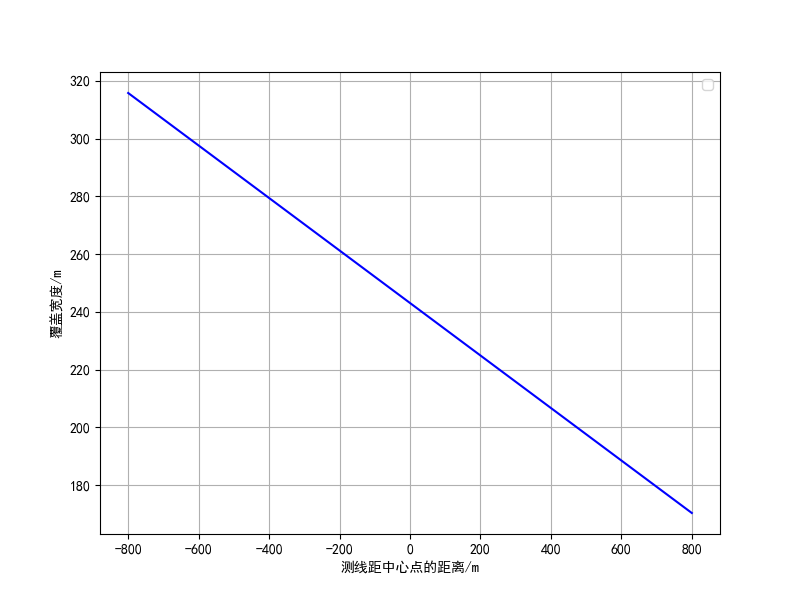
\includegraphics[width=.5\textwidth]{myplot1.png}
        \caption{问题一覆盖宽度随测线距海域中心点处的距离变化图像}
        \label{6}
    \end{figure}

    % \begin{figure}[htbp]
    %     \centering
    %     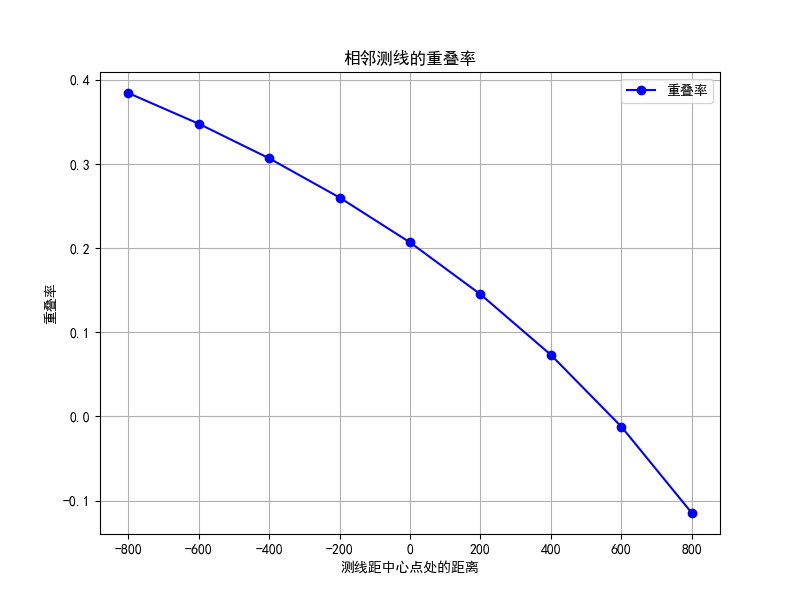
\includegraphics[width=.8\textwidth]{myplot2.png}
    %     \caption{问题一重叠率随测线距海域中心点处的距离变化图像}
    %     \label{7}
    % \end{figure}

    在深入观察图表数据后,可以明显地识别出一系列重要的趋势和关联。

    首先,随着测线距离海域中心点的增加,覆盖宽度逐渐减小。这一结果清晰地表明,在海域中心附近,测线能够覆盖更广泛的地理区域,但随着距离的增加,测线的覆盖范围逐渐减小。这个趋势可能是由于测线靠近海域中心点时,其探测范围更广泛,因此能够覆盖更多的地理区域。然而,一旦远离海域中心,测线的探测范围会逐渐减小,导致覆盖宽度减小。
    
    其次,覆盖宽度与测线距离海域中心点的距离之间存在明显的线性关系。这意味着随着测线距离的增加,覆盖宽度以某种线性方式减小。这种线性关系可能反映了海域的地理特征以及测线在不同距离下的探测性能变化。
    
    

    \section{问题二模型建立与求解}
    \subsection{多波束测线三维立体模型}
    在实际情况中,多波束测探系统通过连续的测量沿着航迹运动,逐点获取数据,以揭示真实的海底情况。
    通过发射多个声波束,这些声波束以不同的角度朝向海底。当这些声波束与海底或水下物体相互作用时,它们会反射回测探系统,从而生成回波数据。
    通过分析回波数据,我们可以确定水深、海底地形的高程、水下物体的位置和尺寸。
    对于一个矩形待测海域,测线方向与海底坡面的法向在水平面上投影的夹角为$\beta$,其坡度为$\alpha$,海域中心点处海水深度为$D$。
    以垂直于水平面方向为$Z$轴,以海底坡面的法向在水平面的投影为$X$轴,以坡面法向与水平面法向组成的平面法向方向为$Y$轴,建立如图~\ref{8}所示的坐标系,证明详见附录一。
    
    \begin{figure}htbp]
        \centering
        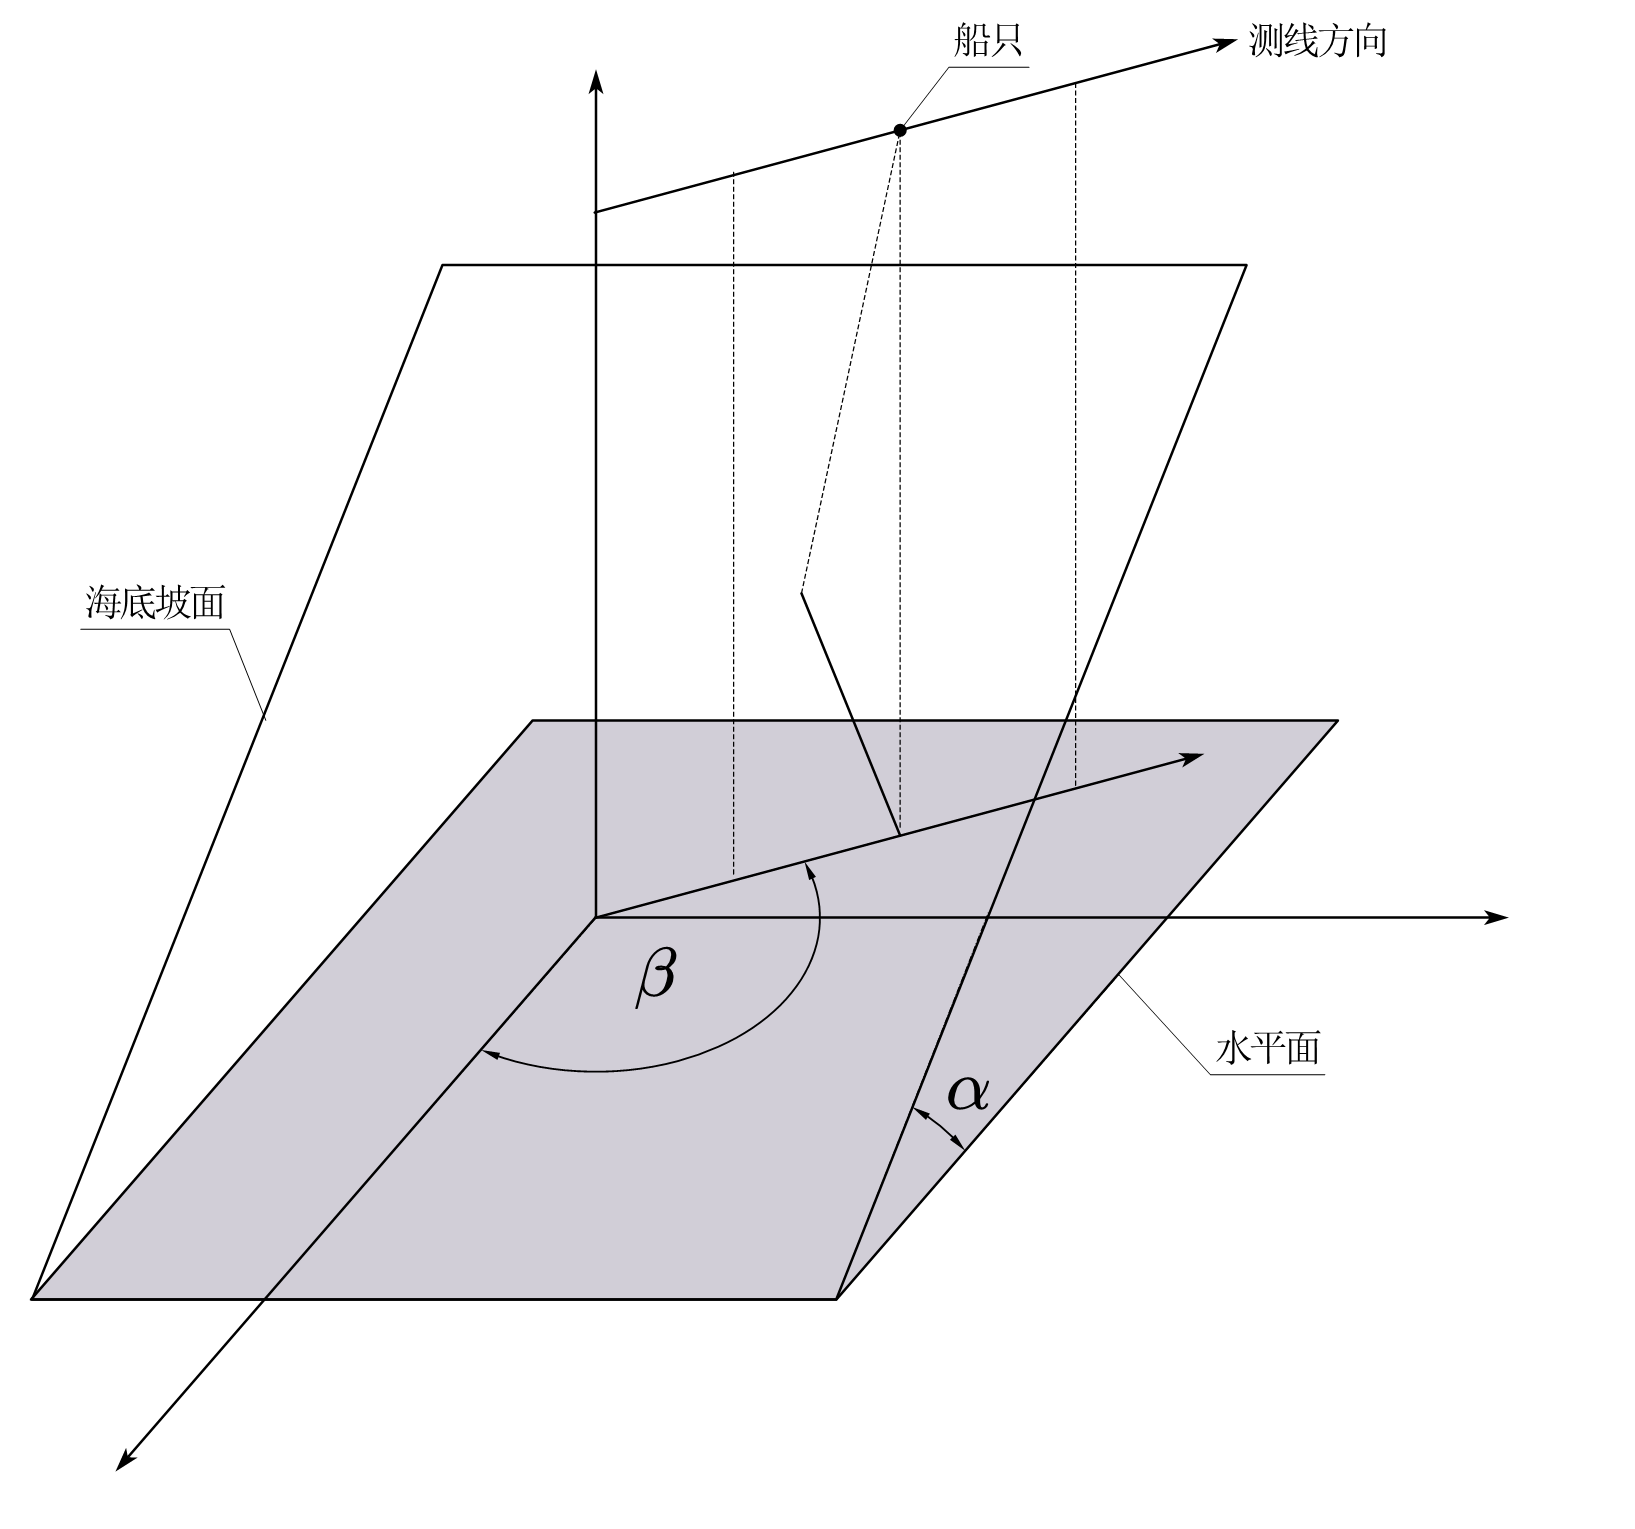
\includegraphics[width=.6\textwidth]{矩形多波束.png}
        \caption{多波束测线三维示意图}
        \label{8}
    \end{figure}

    % \begin{figure}[htbp]
    %     \centering
    %     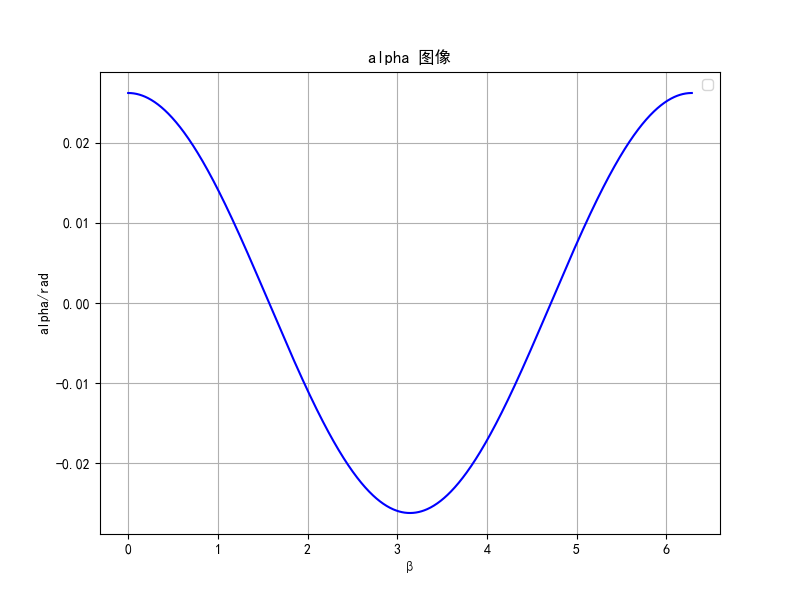
\includegraphics[width=.5\textwidth]{alpha.png}
    %     \caption{$\alpha$坡度图像}
    %     \label{9}
    % \end{figure}

    对于沿测线方向每点探测的覆盖宽度 $W(x)$将其分解为$X$方向$W_X(x)$和$Y$方向$W_Y(x)$ 。
    将测线方向与$Y$轴所夹的锐角,记为$\theta_1$,其可用$\beta$表示。
    $\theta_1$ 随投影的夹角 $\beta$ 的变化情况如图~\ref{10}所示
    \begin{figure}[htbp]
        \begin{minipage}{0.5\textwidth}
            \begin{equation}
                \theta_1 = \begin{cases}
                    \beta & 0 \leq \beta \leq \frac{1}{2} \pi \\
                    \pi - \beta & \frac{1}{2} \pi \leq \beta \leq \pi \\
                    \beta - \pi & \pi \leq \beta \leq \frac{3}{2} \pi \\
                    2\pi - \beta & \frac{3}{2} \pi \leq \beta \leq 2\pi
                \end{cases}
            \end{equation}
        \end{minipage}
        \begin{minipage}{0.5\textwidth}
            \centering
            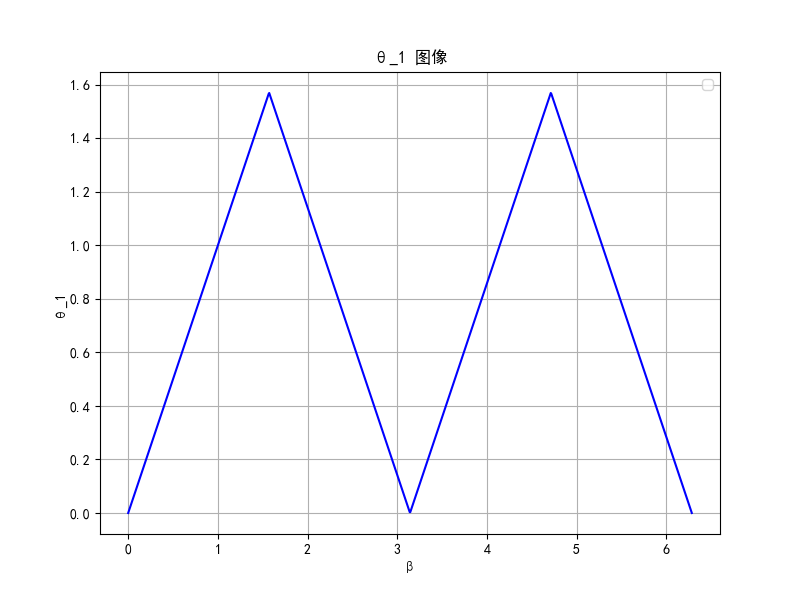
\includegraphics[width=\textwidth]{第二问1.png}
            \caption{$\theta_1$图像}
            \label{10}
        \end{minipage}
    \end{figure}
    
    \begin{figure}[htbp]
        \centering
        
\includegraphics[width=.4\textwidth]{分解示意图.png}
        \caption{测线移动分解示意图}
        \label{11}
    \end{figure}

    同时将相对于起始点的位移分解为$x_{x}、x_{y}$,$x_{x}$仅会影响$W_Y(x)$的长度,
    $x_{y}$仅会影响$W_X(x)$的长度,原理如图~\ref{11}~所示。位移x沿$Y$方向的位移分量$x_y$和沿$X$位移分量$x_x$可表示为


    \begin{equation}
        \left\{
        \begin{aligned}
            &x_x=x |\cos \theta_1|\\
            &x_y=x |\sin \theta_1|
        \end{aligned}
        \right.
    \end{equation}


    $W(x)$沿$Y$方向$W_Y(x)$由公式\ref{eq1}计算得到
    \begin{equation}
        W_Y(x)=\frac{D(x) \sin{(\frac{\theta}{2}})}{\cos{(\alpha-\frac{\theta}{2}})}+\frac{D(x) \sin{(\frac{\theta}{2}})}{\cos{(\alpha+\frac{\theta}{2}})}
        \label{eq4}
    \end{equation} 
    其中$D(x)$是测线方向测量船距海域中心点处距离为$x$时的海水深度。
    $W(x)$沿$X$方向$W_X(x)$由公式\ref{eq1}计算得到
    \begin{equation}
        W_X(x)=2 \times x_x\times \tan{\frac{\theta}{2}}
    \end{equation}
    其中$D_0$表示测线起始位置时的海水深度。
   

    \begin{figure}[htbp]
        \centering
        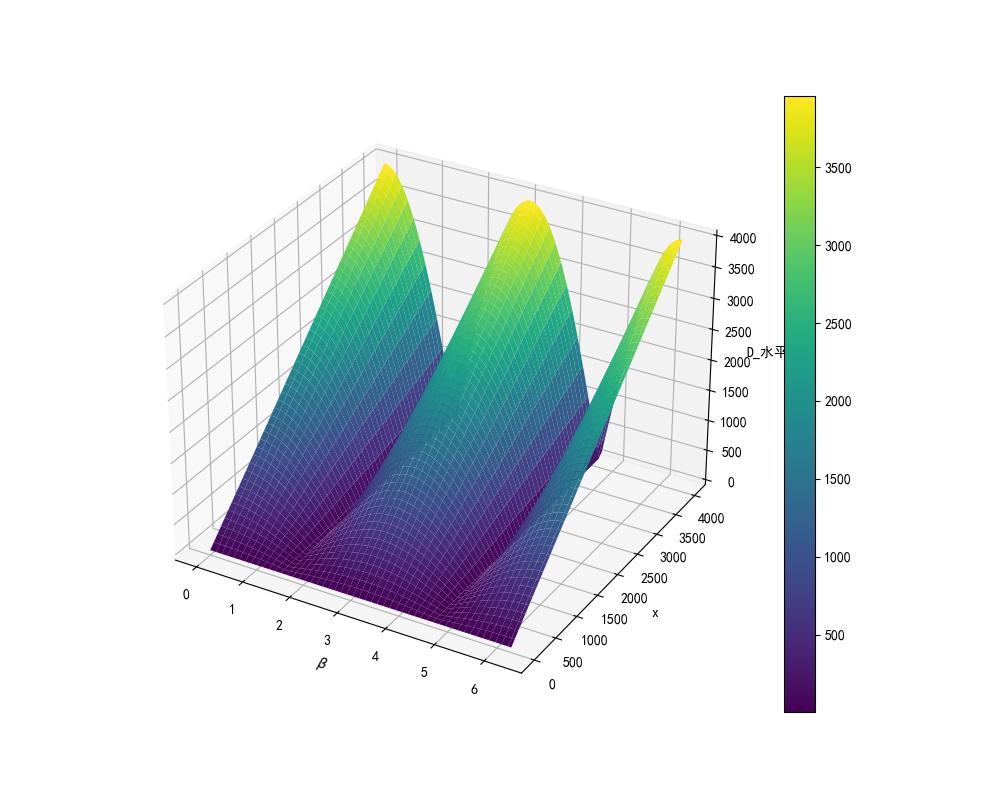
\includegraphics[width=.6\textwidth]{第二问2.png}
        \caption{$x_x$图像}
        \label{12}
    \end{figure}
    
    根据公式\ref{eq3},$D(x)$可表示为
    \begin{equation}
        D(x)=D_0-x_x\tan{\alpha}
        \label{eq5}
    \end{equation}
    $x_x$图像如图~\ref{12}所示。
    联立公式\ref{eq4},\ref{eq5}得   
    \begin{equation}
        W_{\text {总 }}=\sqrt{W_Y^2+W_X^2(x)}
    \end{equation}

    \subsection{问题二模型求解}
    本部分将对上述三维模型进行求解。计算流程如下图所示:
    \begin{figure}[htbp]
        \centering
        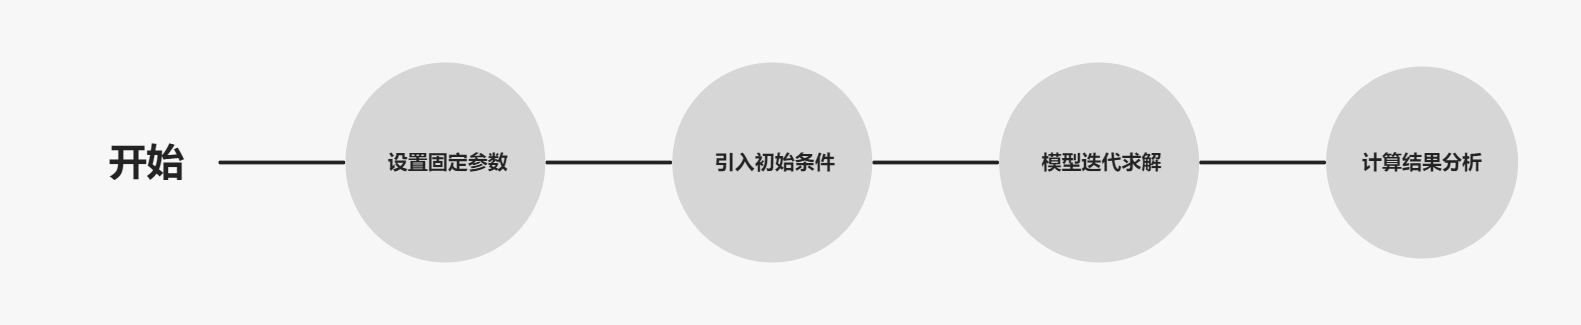
\includegraphics[height=0.1\textheight]{开始.png}
        \caption{问题二计算流程图}
        \label{14}
    \end{figure}
    
    \textbf{1.固定参数}
    在进行多波束测线三维立体模型的结果计算时,需要考虑题目中提供的参数,这些参数在求解过程中保持不变。这些参数包括:
    \begin{itemize}
        \item 海域的几何形状和大小。
        \item 海域中心点处的海水深度$D$。
        \item 海底坡度$\alpha$。
        \item 声波束的发射角度范围。
    \end{itemize}
    这些固定参数对于模型的求解和结果分析至关重要,它们将影响最终的优化结果。
    
    \textbf{2.初始条件}
    在开始数值优化过程之前,同时也需要设定一些初始条件,以便算法能够正常运行。这些初始条件包括:
    \begin{itemize}
        \item 测线方向夹角。
        \item 测量船距海域中心点处的距离。
        \item 算法的迭代步长。
    \end{itemize}
    
    \textbf{3.模型求解策略}
    针对第二问,其所求结果覆盖宽度被表达为一个二元函数,故对两自变量交替迭代最准得到计算结果。
    \begin{algorithm}
        \caption{计算 wx, wy 和 w 的值}
        \begin{algorithmic}[1]
        \Procedure{Theta}{$\beta$}
            \If{$0 < \beta \leq 0.5 \cdot \pi$}
                \State \Return $\beta$
            \ElsIf{$0.5 \cdot \pi < \beta \leq \pi$}
                \State \Return $\pi - \beta$
            \ElsIf{$\pi < \beta \leq 1.5 \cdot \pi$}
                \State \Return $\beta - \pi$
            \ElsIf{$1.5 \cdot \pi < \beta \leq 2 \cdot \pi$}
                \State \Return $2 \cdot \pi - \beta$
            \EndIf
        \EndProcedure
        
        \State 设置 q, beta, m, a, theta, x, d0 和 alpha 的值
        \State 计算$w_0$ 、$w_y$ 、 $w_x$ 、$\theta_x$ 、 $\theta_y$ $d$ 、 $d_1$、$w_y$ 、 $w_x$ 、 $w$
        \State 打印 wx, wy, w
        \end{algorithmic}
    \end{algorithm}
        

    \textbf{4.结果分析}
    问题二计算结果如下表所示:
    \begin{table}[htbp]
        \caption{问题二的计算结果}
        \centering
        \begin{tabular}{cc|cccccccc}
            \toprule[2pt]
            \multirow{2}{*}{覆盖宽度/m} & \multicolumn{8}{c}{测量船距海域中心点处的距离/海里}  \\
            \cmidrule(lr){3-10}
             & & 0 & 0.3 & 0.6 & 0.9 & 1.2 & 1.5 & 1.8 & 2.1 \\
            \midrule[1pt]
             & 0 & 415.7 & 466.1 & 516.5 & 566.9 & 617.3 & 667.7 & 718.1 & 768.5 \\
             & 45 & 416.2 & 451.9 & 487.5 & 523.2 & 558.9 & 594.6 & 630.2 & 665.9 \\
            测线 & 90 & 416.7 & 416.7 & 416.7 & 416.7 & 416.7 & 416.7 & 416.7 & 416.7 \\
            方向 & 135 & 416.2 & 380.5 & 344.8 & 309.2 & 273.5 & 237.8 & 202.1 & 166.5 \\
            夹角 & 180 & 415.7 & 365.3 & 314.9 & 264.5 & 214.1 & 163.7 & 113.3 & 62.9\\
            /$^\circ$ & 225 & 416.2 & 380.5 & 344.8 & 309.2 & 273.5 & 237.8 & 202.1 & 166.5 \\
             & 270 & 416.7 & 416.7 & 416.7 & 416.7 & 416.7 & 416.7 & 416.7 & 416.7 \\
             & 315 & 416.2 & 451.9 & 487.5 & 523.2 & 558.9 & 594.6 & 630.2 & 665.9 \\
            \bottomrule[2pt]
        \end{tabular}
    \end{table}
    
    将所得到的$W(x)$的计算结果绘制成图像,如图\ref{15}所示。
    
    \begin{figure}[htbp]
        \centering
        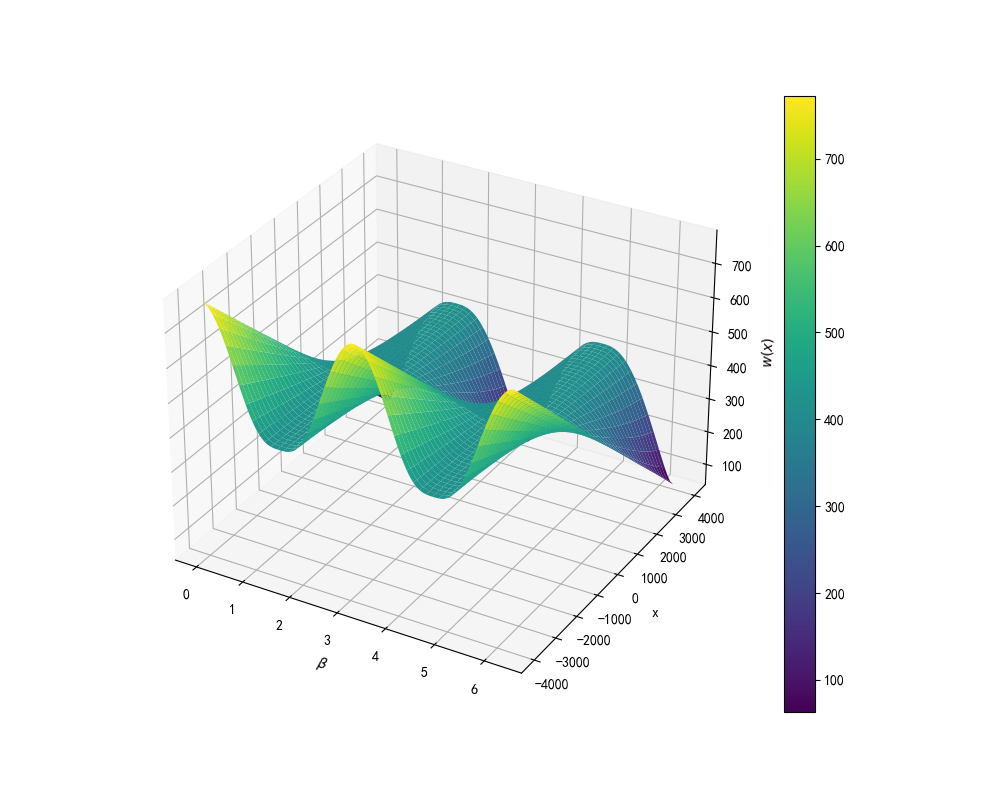
\includegraphics[width=0.6\textwidth]{第二问4.png}
        \caption{第二问的解图像}
        \label{15}
    \end{figure}
    
    \section{问题三模型建立与求解}
    \subsection{多波束测线三维优化指标的提出}
    依据已建立的多波束测线三维立体模型,对于一个坡度为$\alpha$的斜坡,可以得到沿测线方向每点探测的覆盖宽度$W(x)$, 则对于从$\alpha$到$\beta$的测线$L_{AB}$多波束测线覆盖面积$S(x)$可以表示为
    \begin{equation}
        S(x)=\int W(x) d x
    \end{equation}
    所以测线$L_{AB}$在沿测线方向上单位距离扫描增益$S_x(x)$可以表示为
    \begin{equation}
        S_x(x)=\frac{\int_a^b W(x) d x}{l_{AB}}
    \end{equation}
   其中$\alpha$、$\beta$分别为测线$L_{AB}$的起始点和终止点,$l_{AB}$为测线$L_{AB}$的长度。不难看出单位距离扫描增益$S_x(x)$为$\alpha$、$\beta$、$\beta$的函数
  

   
   \subsection{多波束测线三维优化模型的建立}
   综上,多波束测线三维优化模型可表示为
   \begin{gather}
       \quad \min\sum_{i=1}^{n} x_{i} \\
       \text { s.t. }\left\{\begin{array}{l}
           i=\left\lceil\frac{l \sin \left(\frac{3}{2} \pi-\alpha-\beta\right)}{d}\right\rceil \\
           0 \leq \beta \leq 2 \pi\\
               10\% \leq \eta \leq 20\%                    \\	
       \end{array}\right.
   \end{gather}

   对于一宽度为$W_M$, 长度为$L_M$,坡度为$\alpha$的举行待测海域,其三维测线覆盖率可表示为
   \begin{equation}
   \eta_{\text {三维 }}=\frac{\int W_{\text {重 }} d_x \times 2}{\int W_{\text {测 } 1} d_x+\int W_{\text {测 } 2} d_x}
\end{equation}

 
   \begin{figure}[htbp]
    \centering
    \begin{minipage}[c]{0.48\textwidth}
        \centering
        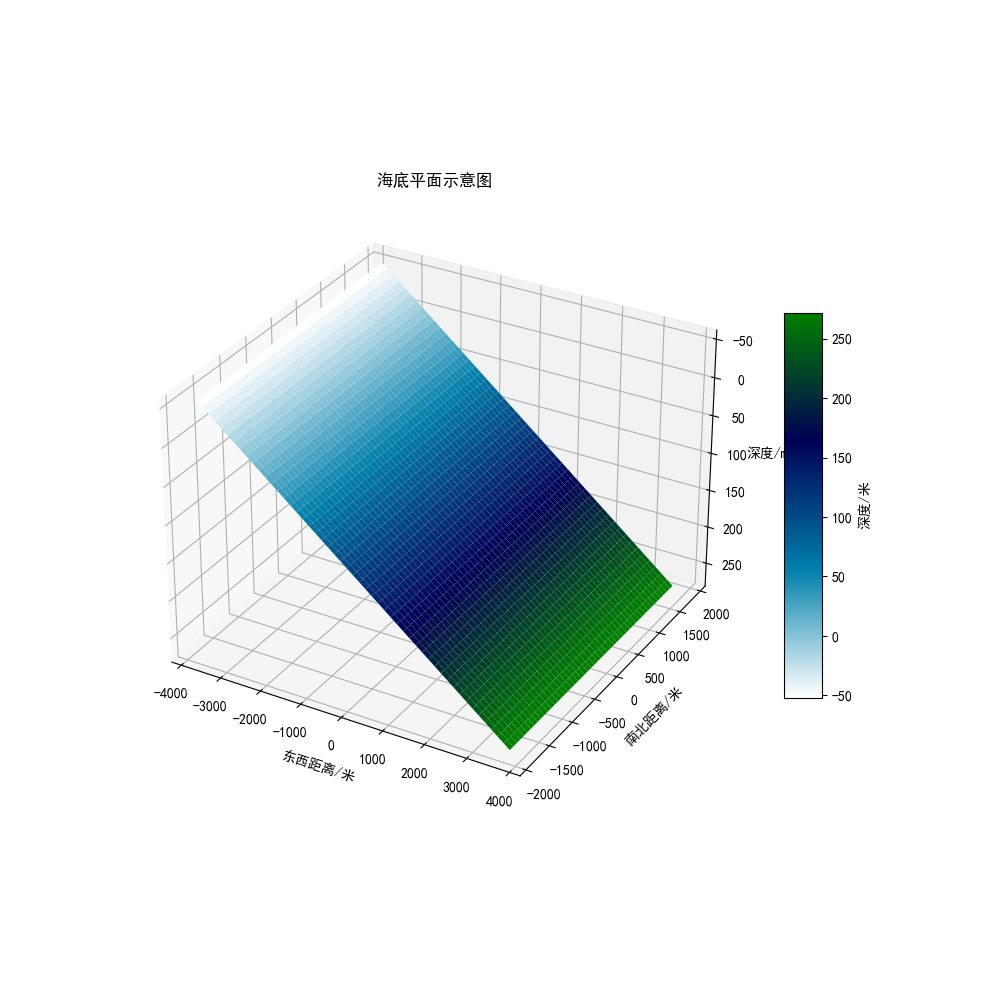
\includegraphics[height=0.3\textheight]{海底图.png}
        \subcaption{海海底坡面深度示意图}
        \label{16}
    \end{minipage}
    \begin{minipage}[c]{0.48\textwidth}
        \centering
        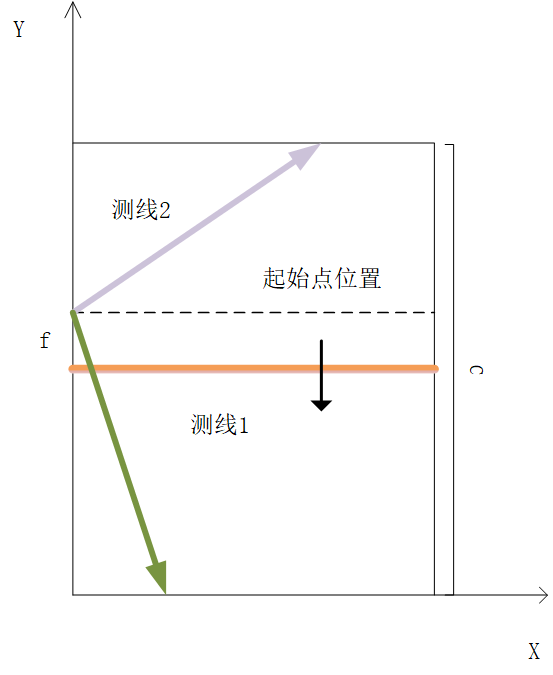
\includegraphics[height=0.3\textheight]{第三问2.png}
        \subcaption{测线}
        \label{32}
    \end{minipage}
    \caption{海水示意图}
\end{figure}




    \begin{figure}[htbp]
        \centering
        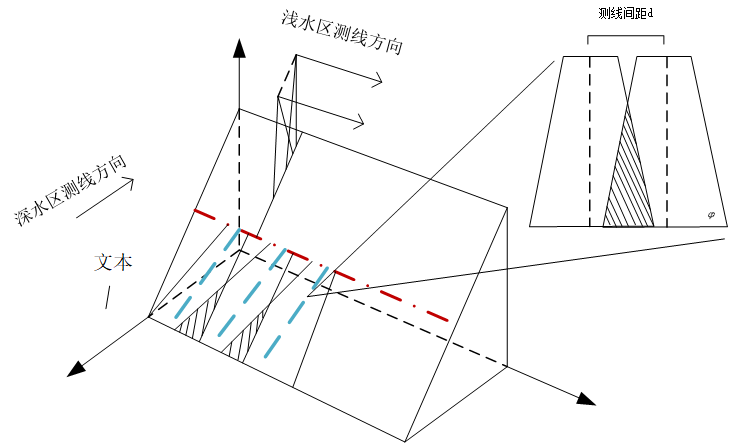
\includegraphics[width=.8\textwidth]{第三问4.png}
        \caption{三维测线方向示意图}
        \label{18}
    \end{figure}



    \subsection{问题三模型求解}
    对于多波束测线三维优化模型,其中单位距离扫描增益$S_x(x)$为$\alpha$、$\beta$、$\beta$的函数。
    因此为了便于求解问题三,多波束测线三维优化模型被分解成两个子问题,即最优化测线方向和最优化测数量, 要优化问题三
    可以先求解子问题$(1)$, 得到最优角度$\beta$,将$\beta_{max}$带入原模型,求解得到最优测线数量$n$。
    \begin{equation}
        \max_{\beta} arg S_x(x)_{AB}
    \end{equation}

    对于子问题$(1)$,
    在坡度固定为$\alpha$的坡面M中,选取与等深线平行的条形微元$m$,其宽度为$dm$, 对于这样一条,起始点,终止点,宽度均固定的窄带,其单位距离扫描增益$S_x(x)$
    仅为$\beta$的函数。遍历$\beta \in [0,2\pi]$,得到最大的$S_x(x)$,即为最优角度$\beta_{max}$。当$dm$趋近于0时,$\beta_{max}$即为单点最优方向,逐点决策
    ,最终得到最优测线方向。

    为了确定初始位置的选择,在问题三中建立起以南北方向为$X$轴,东西方向为$Y$轴的二维坐标系
    对于沿测线方向上单位距离扫描面积$S_x(x)$,我们先确定起始位置,接着在确定起始位置上的航迹方向上
    \begin{equation}
        \left\{
        \begin{aligned}
            & l_1=\frac{\frac{1}{2} c-f}{\sin \theta_{11}} \\
            & l_2=\frac{\frac{1}{2} c+f}{\cos \theta_{12}}
        \end{aligned}
        \right.
    \end{equation} 
    其中$c$表示矩形海域的坡度变化边边长,$f$表示起始位置距离海域中心点处的距离,$\theta_{11}$表示沿坡度上升方向测迹航向,$\theta_{12}$表示沿坡度下降方向测迹航向



    将子问题$(1)$所解出的$\beta_{max}$,带入三维优化模型中即可确定最优测线数量。
    经过Python代码求解,得到当决策点在中心点下方时最优角度为$\pi$,当决策点在中心点上方时最优角度为$0.5\pi$,最小化测线的总长度为127788m。
    \section{问题四模型建立与求解}
    \begin{figure}[htbp]
        \centering
        \begin{minipage}[c]{0.48\textwidth}
            \centering
            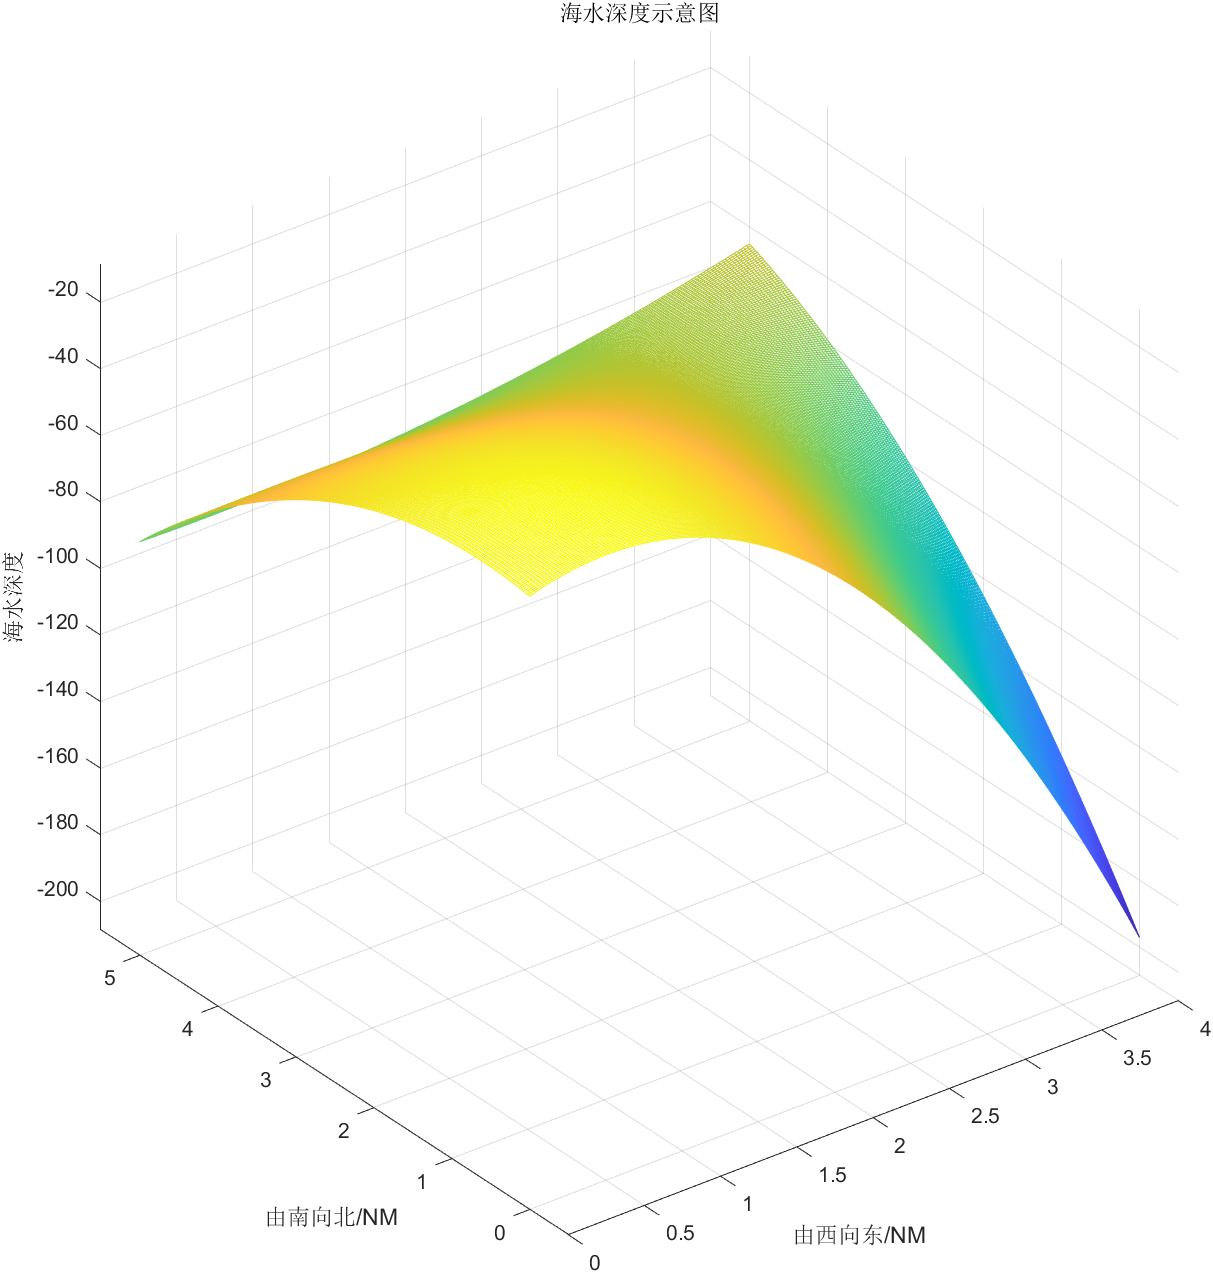
\includegraphics[height=0.3\textheight]{第四问1.png}
            \subcaption{海底深度等深线图}
            \label{20}
        \end{minipage}
        \begin{minipage}[c]{0.48\textwidth}
            \centering
            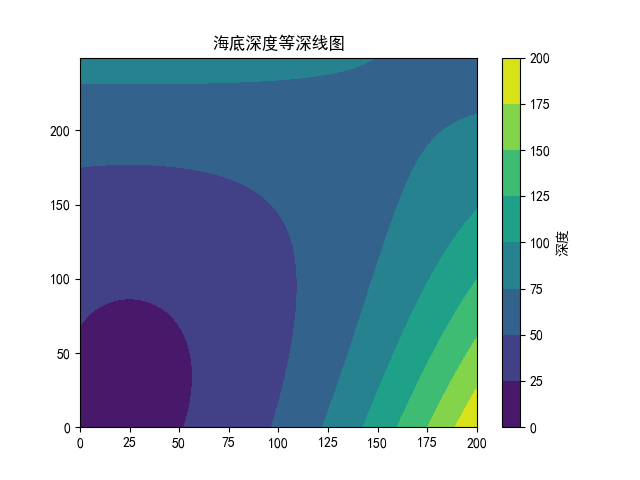
\includegraphics[height=0.3\textheight]{第四问2.png}
            \subcaption{海水深度示意图}
            \label{32}
        \end{minipage}
        \caption{海水深度}
    \end{figure}

    前文已经针对固定坡度的海底坡面,建立了多波束测线三维立体模型和多波束测线三维优化模型,但是在实际情况中,海底坡面的坡度并不是固定的,
    而是随着位置的变化而变化的。已建立的模型并不能完全适用于任意海域的多波束侧线的设计
    因此,本部分在前文所建立模型上提出了任意海域多波束测线设计方法
    \subsection{问题四模型建立}
        对于一海底坡度变化的不规则的任意矩形待测海域,根据微元法对其进行离散化处理,
        将其分解为若干个面积相同的的矩形平面海域,对于每个矩形海域,使用其中心点深度近似其整体深度,
        以此建立多波束测线三维立体模型,对于每个矩形海域,使用多波束测线三维优化模型进行优化,
        最后使微元面积趋近于0,进行逐点决策。
     
               \subsection{问题四模型求解}

                
   

               根据附件 海水深度数据中的数据,利用Python画出海水深度等深线图如图~\ref{20}所示,海水深度示意图如图~\ref{32}所示。
               首先,将附件中提供的数据组为中心点,对该海域进行离散化处理,以0.02海里作为间隔,
               第二,设计指标以满足指标:1.尽可能的覆盖整个待测海域,2.相邻条带重叠率尽量低于$20\%$, 3.测线总长度尽可能短。 
               其次,选定$(0,0)$中心点作为起始点,遍历所有点,计算出每个点的覆盖宽度,重叠率,以此作为指标进行决策。
               最终,根据每点决策生产测线轨迹。其结果如图~\ref{19}所示。

               \begin{figure}[htbp]
                \centering
                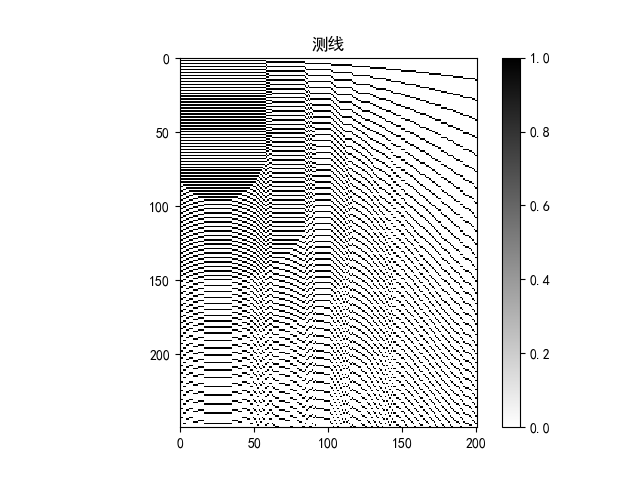
\includegraphics[width=.7\textwidth]{第三问答案.png}
                \caption{第四问的解}
                \label{19}
            \end{figure}
               按照图~\ref{19}所示测线,其指标如下表所示:
    \begin{table}[!htbp]
        \caption{问题四的计算结果} 
        \centering
        \begin{tabular}{ccc}
            \toprule[2pt]
            测线总长度/m & 漏测海区占总待测海域面积的百分比 & 重叠率超过20\%的测线总长度 \\
            \midrule[1pt]
            441183.44 & 0.06837 & 3000.24\\
            \bottomrule[2pt]
        \end{tabular}
    \end{table}
    
   
    
    \section{灵敏性分析}
    \subsection{灵敏性分析}
    根据问题二的分析,可以明显看出,诸如 $D(x)$ 和相邻重叠率等变量对因变量有显著影响。因此,我们在问题二中对 $D(x)$ 和相邻重叠率进行了灵敏度分析,使它们的值产生轻微波动。我们绘制了相邻重叠率随测线距中心点距离的变化情况,如图~\ref{34}所示。 
    随着距离的增加,重叠率呈现出逐渐减小的凸函数形状。这意味着在较短的距离范围内,重叠减少的速度相对较慢,两个对象或现象之间仍然存在较高的重叠度。然而,随着距离逐渐增加,重叠率的减小速度加快,导致它们之间的共同部分逐渐减少。
    这个凸函数趋势反映了距离对于重叠率的影响:当距离较近时,相似性或共同性仍然存在,因此重叠率逐渐减小。但随着距离的增加,这种相似性逐渐减弱,导致重叠率减小速度加快,最终趋向于较低的数值。
    这说明在一定范围内,相邻测线重叠率对于测线距离海域中心点的距离不敏感。但是,当距离超过一定范围时,相邻测线重叠率对于测线距离海域中心点的距离变得敏感。
    
    \begin{figure}[htbp]
        \centering
        \begin{minipage}[c]{0.48\textwidth}
            \centering
            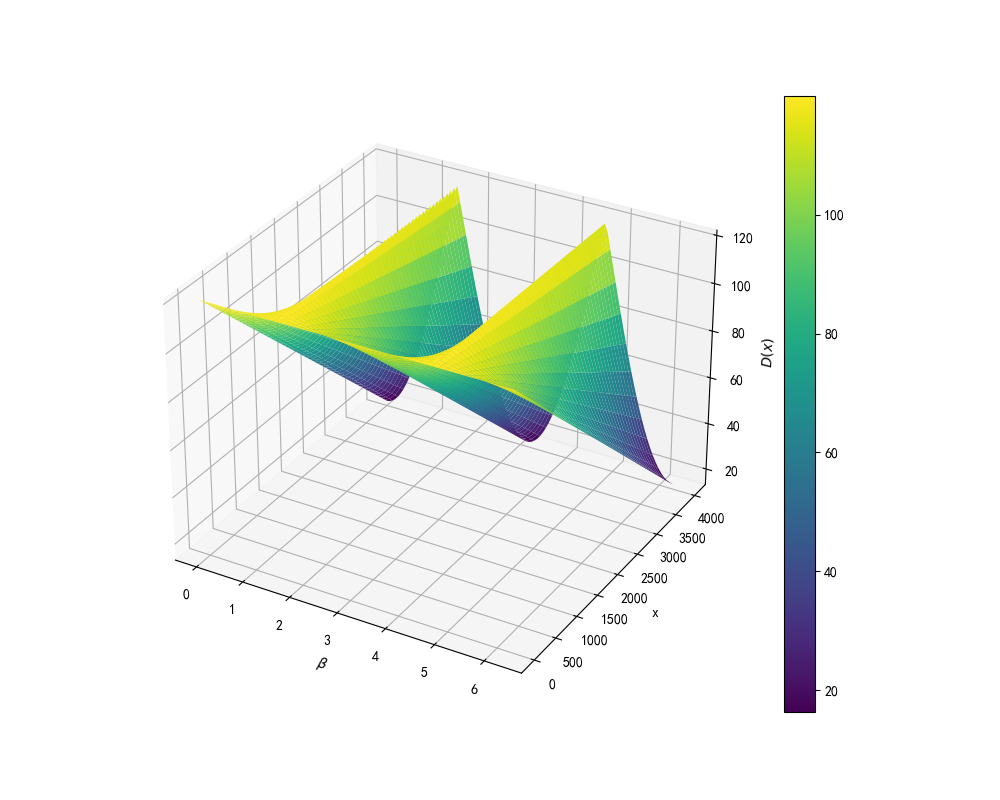
\includegraphics[height=0.3\textheight]{第二问3.png}
            \subcaption{$D(x)$ 灵敏度分析}
            \label{20}
        \end{minipage}
        \begin{minipage}[c]{0.48\textwidth}
            \centering
            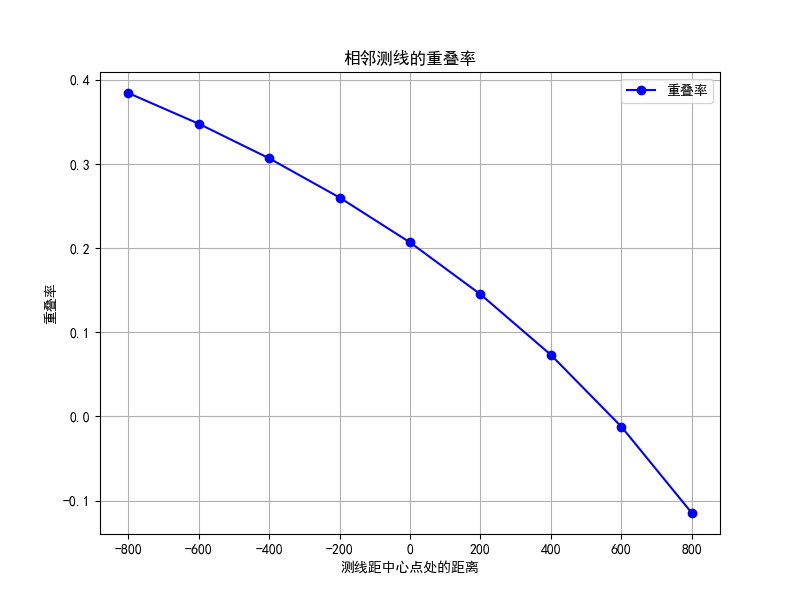
\includegraphics[height=0.26\textheight]{myplot2.png}
            \subcaption{相邻重叠率的灵敏度分析}
            \label{34}
        \end{minipage}
        \caption{灵敏度分析}
    \end{figure}
    
    \subsection{误差分析}
    如问题二所述,$\alpha$ 存在一定的不可避免误差。因此,我们对问题二中的 $\alpha$ 进行了误差分析,使其值产生轻微波动。我们绘制了 $\alpha$ 随 $\beta$ 变化的情况,如图~\ref{21}所示。
    关于 $\alpha$ 随 $\beta$ 的变化情况如下:
    当 $\beta$ 较小时,$\alpha$ 变化较慢,呈现出逐渐的趋势。
    随着 $\beta$ 的增加,$\alpha$ 开始迅速增加,达到一个峰值。
    然后,随着 $\beta$ 的继续增加,$\alpha$ 的增长速度减慢,但仍保持在相对高的水平。
    最后,当 $\beta$ 非常大时,$\alpha$ 的增长速度再次变得较慢,甚至可能出现下降的趋势。
    这种变化可以解释为当 $\beta$ 较小时,$\alpha$ 受到较少的限制,因此增长较为平缓。当 $\beta$ 逐渐增大时,对 $\alpha$ 的限制开始显现,导致增长迅速,但随后受到限制的影响逐渐增强,导致增长速度减慢。最终,当 $\beta$ 达到一定阈值时,限制变得显著,导致 $\alpha$ 的增长再次减慢甚至下降。
    只有当 $\beta$ 处于适中的范围时,$\alpha$ 的变化才相对稳定,不会出现极端的增长或下降情况。
    
    \begin{figure}[htbp]
        \centering
        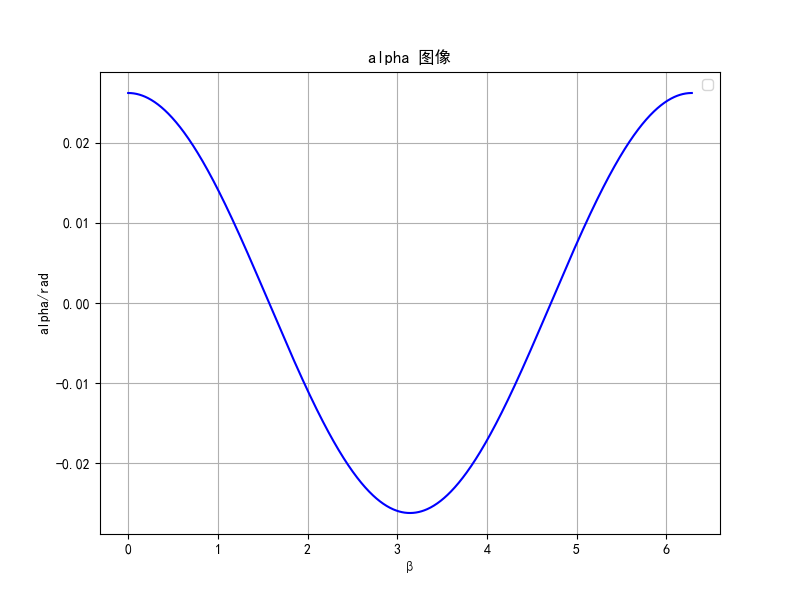
\includegraphics[width=.6\textwidth]{alpha.png}
        \caption{$\alpha$坡度}
        \label{21}
    \end{figure}

    \section{模型评价}
    \subsection{模型优点}
    \begin{enumerate}
        \item \textbf{多波束测线二维平面模型:适用性广泛}考虑了不同位置的水深变化和测量船的水平位移,提供了一种较为通用的方法来计算覆盖宽度和重叠率。
        因此,它适用于不同的海底地理条件,可以应对不同地理条件下的测量任务,适用性较强。
        \item \textbf{多波束测线三维立体模型:精确地形建模}该模型考虑了海底坡面的三维结构,能够更精确地建模复杂的海底地形。
        这对于需要高精度地形数据的应用非常有价值,例如海底地质研究和资源勘查等研究活动。
    \end{enumerate} 
    \subsection{模型缺点}
    \begin{enumerate}
        \item 问题一中二维模型,考虑影响因素较少,只考虑了海底坡度的影响,没有考虑海底地形的复杂性,因此在实际应用中可能会出现一定的误差,模型精度较差。
        \item 本问题讨论的均为静态的模型,不涉及时间相关量,缺乏对动态因素的考察以及其优化结果往往不具有可操作性。
    \end{enumerate} 
    \subsection{模型改进与推广}
    为解决水下探测中所遇到的各种情况, 多波束测深系统应用了先进的测量技术,设备在不同海水环境中测量的误差, 直接关系到测深的精度,在实际工程运用中应当考虑环境对声速的影响,即声速误差:水体物理性质的变化, 主要是水温、盐度、浑浊度的变化造成的水体密度变化, 造成声波在水中的旅行路线弯曲怪异, 引起每个水深点的误差。
    查阅资料得声速$c$是声波在水中传播的速度,它可以用以下近似公式计算:
    \begin{equation}
        C=1449.2+4.6 T-0.055 T^2+0.00029 T^3+(1.34-0.01 T)(S-35)+0.016 Z
    \end{equation}
    其中:$\mathrm{T}$ 是水的温度(单位为摄氏度),$S$ 是水的盐度(以盐度单位表  示,通常以PSU或practical salinity units表示),$\mathrm{Z}$ 是水的深度 (以米表示)。

    声波散射和吸收:声波在水中传播时会与水中的悬浮颗粒物相互作用,导致散射和吸收。这些过程的详细描述需要考虑颗粒物的大小、浓度和声波频率等因素,通常需要复杂的数学模型来描述。


    \section{参考文献}
    \begin{thebibliography}{99} % 如果有超过10个参考文献,请将9替换为99以适应更多的数字

        \bibitem{bib:one} 朱庆, 李德仁. 多波束测深数据的误差分析与处理[D]. 1998.
    
        \bibitem{bib:two} 陆秀平等. 浅水多波束测深潮汐改正技术研究[D]. 2008.
    
        \bibitem{bib:three} 李治远, 豆虎林, 张海泉. SeaBeam全海深多波束测深系统及应用[J]. 海岸工程, 2021, 40(1): 59-67.
    
        \bibitem{bib:four} 沈蔚等. 深水多波束测深系统测深精度评估[J]. 海洋测绘, 2020, 40(3): 19-23.
    
    \end{thebibliography}  
    
    \newpage
    \section{附录一}
    \begin{figure}[h]
        \centering
        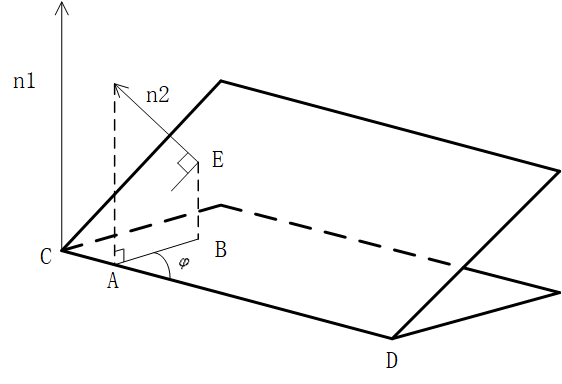
\includegraphics[scale=0.9]{21}
        \caption{证明图}
        \label{31}
    \end{figure}
    
    由图\ref{31}~可以得到直线$CD$是坡面与水平面的交线, $n_1$为水平面的法向量,$n_2$为坡面的法向量,直线 $AB$是坡面法线$n_2$在水平面上的投影与直线$CD$相交于点$\alpha$。因为$n_2$是坡面的法向量,可以推出$n_2$垂直玉坡面,又因为$CD$属于坡面,所以$n_2$垂直于$CD$。同理可得直线$CD$垂直与$n_1$,显然,对法向量$n_1$进行平移,与直线$AB$和法向量$n2$共同构成平面$ABE$。依据直线与平面垂直判定定理:一条直线与一个平面内的两条相交直线都垂直,则该直线与此平面垂直,可以得到直线$CD$垂直于平面$ABE$。又因为直线$AB$属于平面$ABE$,所以我们得出结论,直线$AB$垂直于直线$CD$。据此,我们建立了如图(8)所示的坐标系。
    \section{附录二}
    \begin{appendices}
        \begin{lstlisting}[language=Matlab]
            % D(x)图像代码
            import numpy as np
            import matplotlib.pyplot as plt
            from mpl_toolkits.mplot3d import Axes3D
            plt.rcParams['font.sans-serif']=['SimHei']
            plt.rcParams['axes.unicode_minus'] = False
            # 创建x和y的网格
            x = np.linspace(0, 4200, 100)  # 选择适当的x范围
            y = np.linspace(0, 2 * np.pi, 100)  # 选择适当的y范围
            X, Y = np.meshgrid(x, y)

            # 计算函数值
            d = 120-X * np.sin(np.abs(np.pi - Y))*np.tan(1.5*np.pi/180)

            # 创建三维图形
            fig = plt.figure(figsize=(10, 8))
            ax = fig.add_subplot(111, projection='3d')

            # 绘制三维曲面
            surf = ax.plot_surface(X, Y, d, cmap='viridis')

            # 添加颜色条
            fig.colorbar(surf, ax=ax, label='D(x)')

            # 设置轴标签和标题
            ax.set_xlabel('x')
            ax.set_ylabel('beta')
            ax.set_zlabel('D(x)')
            ax.set_title('D(x)图像')

            # 显示图形
            plt.show()

            % 海底深度三维表面绘图代码
            import pandas as pd
            import matplotlib.pyplot as plt
            from mpl_toolkits.mplot3d import Axes3D

            # 读取Excel文件
            excel_file = r"C:\Users\Lenovo\Desktop\国赛\CUMCM2023Problems\附件.xlsx"
            df = pd.read_excel(excel_file, header=None)

            # 提取数据
            x = df.iloc[1, 2:].values
            y = df.iloc[2:253, 1].values
            z = df.iloc[2:253, 2:]

            # 创建三维表面绘图
            fig = plt.figure()
            ax = fig.add_subplot(111, projection='3d')
            x, y = x[:, None], y[:, None]
            ax.plot_surface(x, y, z, cmap='viridis')

            # 设置坐标轴标签
            ax.set_xlabel('X轴坐标')
            ax.set_ylabel('Y轴坐标')
            ax.set_zlabel('深度')

            # 设置图表标题
            plt.title('海底深度三维表面绘图')

            # 显示图表
            plt.show()
        \end{lstlisting}

        \begin{lstlisting}[language=Python]
            % 问题一求解代码
            import sympy as sp
            import numpy as np

            # 定义符号变量
            x, alpha, beta, theta, D = sp.symbols('x alpha beta theta D')

            # 定义包含NumPy函数的函数
            f = sp.sin(theta/2)*(D-x*sp.sin(sp.Abs(sp.pi-beta))*sp.tan(alpha))/sp.cos(alpha-theta/2) + sp.sin(theta/2)*(D-x*sp.sin(sp.Abs(sp.pi-beta))*sp.tan(alpha))/sp.cos(alpha+theta/2)

            # 求解不定积分
            indefinite_integral = sp.integrate(f, x)

            print(indefinite_integral)

            f_2=indefinite_integral/x

            print(f_2)

            derivative = sp.diff(f_2, x)

            print(derivative)

            x^2 \left( -\frac{\sin\left(\frac{\theta}{2}\right) \sin\left| \beta - \pi \right| \tan(\alpha)}{2\cos(\alpha + \frac{\theta}{2})} - \frac{\sin\left(\frac{\theta}{2}\right) \sin\left| \beta - \pi \right| \tan(\alpha)}{2\cos(\alpha - \frac{\theta}{2})} \right) + x \left( \frac{D \sin\left(\frac{\theta}{2}\right)}{\cos(\alpha + \frac{\theta}{2})} + \frac{D \sin\left(\frac{\theta}{2}\right)}{\cos(\alpha - \frac{\theta}{2})} \right)

            % $\theta_1$求解代码
            import numpy as np
            import matplotlib.pyplot as plt
            from mpl_toolkits.mplot3d import Axes3D
            plt.rcParams['font.sans-serif'] = ['SimHei']
            plt.rcParams['axes.unicode_minus'] = False
            # 定义θ(β)函数
            def theta(beta):
                if 0 <= beta <= 0.5 * np.pi:
                    return beta
                elif 0.5 * np.pi <= beta <= np.pi:
                    return np.pi - beta
                elif np.pi <= beta <= 1.5 * np.pi:
                    return beta - np.pi
                elif 1.5 * np.pi <= beta <= 2 * np.pi:
                    return 2 * np.pi - beta

            theta=np.pi/2
            x=-800
            d0=91
            alpha=1.5*np.pi/180
            # 计算d值

            w0=d0*np.sin(np.pi/3)/np.cos(1.5*np.pi/180-np.pi/3)+d0*np.sin(np.pi/3)/np.cos(1.5*np.pi/180+np.pi/3)
            wx0=w0*np.cos(theta)
            wy0=w0*np.sin(theta)
            thetax=2*np.arctan(wx0/2/d0)
            thetay=2*np.arctan(wy0/2/d0)
            d = x * np.abs(np.cos(theta))
            d_1=d0-d*np.tan(alpha)
            wy=d0*np.sin(thetay/2)/np.cos(alpha-thetay/2)+d0*np.sin(thetay/2)/np.cos(alpha+thetay/2)
            wx=2*d_1*np.tan(thetax/2)
            w=pow(wx**2+wy**2,1/2)
            print(d,w,wx)


            % $D(x)$求解代码
            import numpy as np
            import matplotlib.pyplot as plt
            from mpl_toolkits.mplot3d import Axes3D
            plt.rcParams['font.sans-serif'] = ['SimHei']
            plt.rcParams['axes.unicode_minus'] = False
            # 定义θ(β)函数
            def theta(beta):
                if 0 <= beta <= 0.5 * np.pi:
                    return beta
                elif 0.5 * np.pi <= beta <= np.pi:
                    return np.pi - beta
                elif np.pi <= beta <= 1.5 * np.pi:
                    return beta - np.pi
                elif 1.5 * np.pi <= beta <= 2 * np.pi:
                    return 2 * np.pi - beta

            # 生成一组β值和x值
            beta_values = np.linspace(0, 2 * np.pi, 100)
            x_values = np.linspace(-4000, 4000, 1000)

            # 创建网格点
            beta_grid, x_grid = np.meshgrid(beta_values, x_values)
            theta_grid = np.vectorize(theta)(beta_grid)
            d0=120
            alpha=1.5*np.pi/180
            # 计算d值
            w0=d0*np.sin(np.pi/3)/np.cos(1.5*np.pi/180-np.pi/3)+d0*np.sin(np.pi/3)/np.cos(1.5*np.pi/180+np.pi/3)
            wx0=w0*np.cos(theta_grid)
            wy0=w0*np.sin(theta_grid)
            thetax=2*np.arctan(wx0/2/d0)
            thetay=2*np.arctan(wy0/2/d0)
            d_grid = x_grid * np.abs(np.cos(theta_grid))
            d_1=d0-d_grid*np.tan(alpha)
            wy=d0*np.sin(thetay/2)/np.cos(alpha-thetay/2)+d0*np.sin(thetay/2)/np.cos(alpha+thetay/2)
            wx=2*d_1*np.tan(thetax/2)
            w=pow(wx**2+wy**2,1/2)




            d_grid=w
            # 创建3D图像
            fig = plt.figure(figsize=(10, 8))
            # 创建三维图形
            fig = plt.figure(figsize=(10, 8))
            ax = fig.add_subplot(111, projection='3d')



            surf=ax.plot_surface(beta_grid, x_grid, d_grid, cmap='viridis')
            ax.set_xlabel(r'$\beta$')
            ax.set_ylabel('x')
            ax.set_zlabel('$w(x)$')



            fig.colorbar(surf, ax=ax)
            plt.show()


        \end{lstlisting}
        \begin{lstlisting}[language=Python]
                    import pandas as pd
        import matplotlib.pyplot as plt
        from mpl_toolkits.mplot3d import Axes3D

        # 读取Excel文件
        excel_file = r"C:\Users\Lenovo\Desktop\国赛\CUMCM2023Problems\附件.xlsx"
        df = pd.read_excel(excel_file, header=None)

        # 提取数据
        x = df.iloc[1, 2:].values
        y = df.iloc[2:253, 1].values
        z = df.iloc[2:253, 2:]

        # 创建三维表面绘图
        fig = plt.figure()
        ax = fig.add_subplot(111, projection='3d')
        x, y = x[:, None], y[:, None]
        ax.plot_surface(x, y, z, cmap='viridis')

        # 设置坐标轴标签
        ax.set_xlabel('X轴坐标')
        ax.set_ylabel('Y轴坐标')
        ax.set_zlabel('深度')

        # 设置图表标题
        plt.title('海底深度三维表面绘图')

        # 显示图表
        plt.show()
        \end{lstlisting}
        \begin{lstlisting}[language=Python]
            import numpy as np

            d=2.1*1852
            h0=120
            l=120/np.tan(1.5*np.pi/180)
            d0=(l-d)*np.tan(1.5*np.pi/180)
            
            print(d0)
            w1=d0*np.sin(np.pi/3)/np.cos(1.5*np.pi/180-np.pi/3)+d0*np.sin(np.pi/3)/np.cos(1.5*np.pi/180+np.pi/3)
            print(w1)
            
            d=-2.1*1852
            h0=120
            l=120/np.tan(1.5*np.pi/180)
            d0=(l-d)*np.tan(1.5*np.pi/180)
            
            print(d0)
            w2=d0*np.sin(np.pi/3)/np.cos(1.5*np.pi/180-np.pi/3)+d0*np.sin(np.pi/3)/np.cos(1.5*np.pi/180+np.pi/3)
            print(w2)
            
            eta=(w1/2+w2/2-200)*2/(w1+w2)
            print(eta)
        \end{lstlisting}    
        \begin{lstlisting}[language=Python]
            import numpy as np
            import matplotlib.pyplot as plt
            plt.rcParams['font.sans-serif'] = ['SimHei']
            plt.rcParams['axes.unicode_minus'] = False
            # 定义一系列d值,从-800到800
            d_values = np.linspace(-800, 800, 9)  # 生成400个均匀分布的d值
            
            # 计算每个d值对应的w1值
            def calculate_w1(d):
                l = 70 / np.tan(1.5 * np.pi / 180)
                d0 = (l - d) * np.tan(1.5 * np.pi / 180)
                w1 = d0 * np.sin(np.pi / 3) / np.cos(1.5 * np.pi / 180 - np.pi / 3) + \
                     d0 * np.sin(np.pi / 3) / np.cos(1.5 * np.pi / 180 + np.pi / 3)
                return w1
            
            w1_values = [calculate_w1(d) for d in d_values]
            
            # 创建图形并绘制曲线
            plt.figure(figsize=(8, 6))
            plt.plot(d_values, w1_values,  color='b')
            plt.xlabel('测线距中心点的距离/m')
            plt.ylabel('覆盖宽度/m')
            
            plt.grid(True)
            plt.legend()
            plt.show()

        \end{lstlisting}  
        \begin{lstlisting}[language=Python]
            import numpy as np
            import matplotlib.pyplot as plt
            
            # 定义一系列d值,从-800到800
            d_values = np.linspace(-800, 800, 9)  # 生成9个均匀分布的d值
            
            # 计算每个d值对应的w1和w2值
            def calculate_w1_w2(d):
                l = 70 / np.tan(1.5 * np.pi / 180)
                d0 = (l - d) * np.tan(1.5 * np.pi / 180)
                w1 = d0 * np.sin(np.pi / 3) / np.cos(1.5 * np.pi / 180 - np.pi / 3) + \
                     d0 * np.sin(np.pi / 3) / np.cos(1.5 * np.pi / 180 + np.pi / 3)
                d1 = (l - d + 200) * np.tan(1.5 * np.pi / 180)
                w2 = d1 * np.sin(np.pi / 3) / np.cos(1.5 * np.pi / 180 - np.pi / 3) + \
                     d1 * np.sin(np.pi / 3) / np.cos(1.5 * np.pi / 180 + np.pi / 3)
                return w1, w2
            
            # 计算每个d值对应的eta值
            def calculate_eta(w1, w2):
                eta = (w1 / 2 + w2 / 2 - 200) * 2 / (w1 + w2)
                return eta
            
            # 计算eta值
            eta_values = [calculate_eta(*calculate_w1_w2(d)) for d in d_values]
            
            # 创建图形并绘制eta的图像
            plt.figure(figsize=(8, 6))
            plt.plot(d_values, eta_values, label='重叠率', color='b', marker='o')
            plt.xlabel('测线距中心点处的距离')
            plt.ylabel('重叠率')
            plt.title('相邻测线的重叠率')
            plt.grid(True)
            plt.legend()
            plt.rcParams['font.sans-serif']=['SimHei']
            plt.rcParams['axes.unicode_minus'] = False
            plt.title('相邻测线的重叠率')
            plt.show()  
        \end{lstlisting}
        \begin{lstlisting}[language=Python]
            import numpy as np
import matplotlib.pyplot as plt
plt.rcParams['font.sans-serif'] = ['SimHei']
plt.rcParams['axes.unicode_minus'] = False
# Create an array of beta values from 0 to 2*pi
beta_values = np.linspace(0, 2 * np.pi, 1000)

# Define a function to calculate theta (theta) based on the given piecewise conditions
def calculate_theta(beta):
    if 0 <= beta <= 0.5 * np.pi:
        return beta
    elif 0.5 * np.pi < beta <= np.pi:
        return np.pi - beta
    elif np.pi < beta <= 1.5 * np.pi:
        return beta - np.pi
    elif 1.5 * np.pi < beta <= 2 * np.pi:
        return 2 * np.pi - beta

# Calculate theta values for each beta value
theta_values = [calculate_theta(beta) for beta in beta_values]

# Create the plot
plt.figure(figsize=(8, 6))
plt.plot(beta_values, theta_values, color='b')
plt.xlabel('β')
plt.ylabel('θ_1')
plt.title('θ_1 图像')
plt.grid(True)
plt.legend()
plt.show()
        \end{lstlisting}
        \begin{lstlisting}[language=Python]
            import numpy as np
import matplotlib.pyplot as plt
from mpl_toolkits.mplot3d import Axes3D
plt.rcParams['font.sans-serif'] = ['SimHei']
plt.rcParams['axes.unicode_minus'] = False
# 定义θ(β)函数
def theta(beta):
    if 0 <= beta <= 0.5 * np.pi:
        return beta
    elif 0.5 * np.pi <= beta <= np.pi:
        return np.pi - beta
    elif np.pi <= beta <= 1.5 * np.pi:
        return beta - np.pi
    elif 1.5 * np.pi <= beta <= 2 * np.pi:
        return 2 * np.pi - beta

# 生成一组β值和x值
beta_values = np.linspace(0, 2 * np.pi, 100)
x_values = np.linspace(-4000, 4000, 1000)

# 创建网格点
beta_grid, x_grid = np.meshgrid(beta_values, x_values)
theta_grid = np.vectorize(theta)(beta_grid)
d0=120
alpha=1.5*np.pi/180
# 计算d值
w0=d0*np.sin(np.pi/3)/np.cos(1.5*np.pi/180-np.pi/3)+d0*np.sin(np.pi/3)/np.cos(1.5*np.pi/180+np.pi/3)
wx0=w0*np.cos(theta_grid)
wy0=w0*np.sin(theta_grid)
thetax=2*np.arctan(wx0/2/d0)
thetay=2*np.arctan(wy0/2/d0)
d_grid = x_grid * np.abs(np.cos(theta_grid))
d_1=d0-d_grid*np.tan(alpha)
wy=d0*np.sin(thetay/2)/np.cos(alpha-thetay/2)+d0*np.sin(thetay/2)/np.cos(alpha+thetay/2)
wx=2*d_1*np.tan(thetax/2)
w=pow(wx**2+wy**2,1/2)




d_grid=w
# 创建3D图像
fig = plt.figure(figsize=(10, 8))
# 创建三维图形
fig = plt.figure(figsize=(10, 8))
ax = fig.add_subplot(111, projection='3d')



surf=ax.plot_surface(beta_grid, x_grid, d_grid, cmap='viridis')
ax.set_xlabel(r'$\beta$')
ax.set_ylabel('x')
ax.set_zlabel('$w(x)$')



fig.colorbar(surf, ax=ax)
plt.show()
        \end{lstlisting}
        \begin{lstlisting}[language=Python]
            import numpy as np
import matplotlib.pyplot as plt
from mpl_toolkits.mplot3d import Axes3D
plt.rcParams['font.sans-serif'] = ['SimHei']
plt.rcParams['axes.unicode_minus'] = False
# 定义θ(β)函数
def theta(beta):
    if 0 < beta <= 0.5 * np.pi:
        return beta
    elif 0.5 * np.pi < beta <= np.pi:
        return np.pi - beta
    elif np.pi < beta <= 1.5 * np.pi:
        return beta - np.pi
    elif 1.5 * np.pi < beta <= 2 * np.pi:
        return 2 * np.pi - beta
q=45
beta=q*np.pi/180
m=1852
a=-2.1
theta=theta(beta)
x=a*m
d0=120
alpha=1.5*np.pi/180

# 计算d值
w0=d0*np.sin(np.pi/3)/np.cos(alpha-np.pi/3)+d0*np.sin(np.pi/3)/np.cos(alpha+np.pi/3)
wy0=w0*np.sin(theta)
wx0=w0*np.cos(theta)
thetax=2*np.arctan(wx0/2/d0)
thetay=2*np.arctan(wy0/2/d0)
d = x * np.cos(theta)
d_1=d0-d*np.tan(alpha)
wy=d_1*np.sin(thetay/2)/np.cos(alpha-thetay/2)+d_1*np.sin(thetay/2)/np.cos(alpha+thetay/2)
wx=2*d_1*np.tan(thetax/2)
w=pow(wx**2+wy**2,1/2)
print(wx,wy,w)
# d_grid=w
        \end{lstlisting}
        \begin{lstlisting}[language=Python]
            import numpy as np
import matplotlib.pyplot as plt
from mpl_toolkits.mplot3d import Axes3D
plt.rcParams['font.sans-serif'] = ['SimHei']
plt.rcParams['axes.unicode_minus'] = False
# 定义θ(β)函数
def theta(beta):
    if 0 < beta <= 0.5 * np.pi:
        return beta
    elif 0.5 * np.pi < beta <= np.pi:
        return np.pi - beta
    elif np.pi < beta <= 1.5 * np.pi:
        return beta - np.pi
    elif 1.5 * np.pi < beta <= 2 * np.pi:
        return 2 * np.pi - beta
q=45
beta=q*np.pi/180
m=1852
a=-2.1
theta=theta(beta)
x=a*m
d0=120
alpha=1.5*np.pi/180

# 计算d值
w0=d0*np.sin(np.pi/3)/np.cos(alpha-np.pi/3)+d0*np.sin(np.pi/3)/np.cos(alpha+np.pi/3)
wy0=w0*np.sin(theta)
wx0=w0*np.cos(theta)
thetax=2*np.arctan(wx0/2/d0)
thetay=2*np.arctan(wy0/2/d0)
d = x * np.cos(theta)
d_1=d0-d*np.tan(alpha)
wy=d_1*np.sin(thetay/2)/np.cos(alpha-thetay/2)+d_1*np.sin(thetay/2)/np.cos(alpha+thetay/2)
wx=2*d_1*np.tan(thetax/2)
w=pow(wx**2+wy**2,1/2)
print(wx,wy,w)
# d_grid=w
            
            

        \end{lstlisting}
        \begin{lstlisting}[language=Python]
            import numpy as np
            import matplotlib.pyplot as plt
            plt.rcParams['font.sans-serif'] = ['SimHei']
            plt.rcParams['axes.unicode_minus'] = False
            # Create an array of beta values from 0 to 2*pi
            beta_values = np.linspace(0, 2 * np.pi, 1000)
            
            # Calculate theta values for each beta value
            theta_values = [np.arcsin(np.sin(1.5*np.pi/180)*np.cos(beta)) for beta in beta_values]
            # Create the plot
            plt.figure(figsize=(8, 6))
            plt.plot(beta_values, theta_values, color='b')
            plt.xlabel('β')
            plt.ylabel('alpha/rad')
            plt.title('alpha 图像')
            plt.grid(True)
            plt.legend()
            plt.show()
        \end{lstlisting}  
        \begin{lstlisting}[language=Python] 
           
import sympy as sp
import numpy as np

# 定义符号变量
x, alpha, beta, theta, D = sp.symbols('x alpha beta theta D')

# 定义包含NumPy函数的函数
f = sp.sin(theta/2)*(D-x*sp.sin(sp.Abs(sp.pi-beta))*sp.tan(alpha))/sp.cos(alpha-theta/2) + sp.sin(theta/2)*(D-x*sp.sin(sp.Abs(sp.pi-beta))*sp.tan(alpha))/sp.cos(alpha+theta/2)

# 求解不定积分
indefinite_integral = sp.integrate(f, x)

print(indefinite_integral)

f_2=indefinite_integral/x

print(f_2)

derivative = sp.diff(f_2, x)

print(derivative)


import matplotlib.pyplot as plt
from mpl_toolkits.mplot3d import Axes3D
import numpy as np
plt.rcParams['font.sans-serif'] = ['SimHei']
plt.rcParams['axes.unicode_minus'] = False
# 定义海底平面的尺寸
length = 2 * 1852  # 南北长
width = 4 * 1852  # 东西宽
center_depth = 110  # 中心深度
slope_angle = 1.5  # 坡度角度

# 创建一个平面海底的网格
x = np.linspace(-width / 2, width / 2, 1000)  # 东西方向
y = np.linspace(-length / 2, length / 2, 1000)  # 南北方向
X, Y = np.meshgrid(x, y)

# 计算海底深度
depth = center_depth + (X / (width / 2)) * slope_angle * center_depth

# 创建三维图形
fig = plt.figure(figsize=(10, 10))
ax = fig.add_subplot(111, projection='3d')

# 绘制海底平面
surf = ax.plot_surface(X, Y, depth, cmap='ocean_r')

# 添加颜色条
cbar = fig.colorbar(surf, ax=ax, shrink=0.5, aspect=10)
cbar.set_label('深度/米')

# 设置坐标轴标签
ax.set_xlabel('东西距离/米')
ax.set_ylabel('南北距离/米')
ax.set_zlabel('深度/m')

# 设置标题
ax.set_title('海底平面示意图')

# 显示图形
plt.gca().invert_zaxis()  # 反转z轴以使深度增加朝下
plt.show()


import numpy as np
d0=120
w0=d0*np.sin(np.pi/3)/np.cos(1.5*np.pi/180-np.pi/3)+d0*np.sin(np.pi/3)/np.cos(1.5*np.pi/180+np.pi/3)
w1=d0*np.sin(np.pi/3)/np.cos(-np.pi/3)+d0*np.sin(np.pi/3)/np.cos(+np.pi/3)
eta=np.abs(w1-w0)/w1
print(eta)



import numpy as np

def theta(beta):
    if 0 < beta <= 0.5 * np.pi:
        return beta
    elif 0.5 * np.pi < beta <= np.pi:
        return np.pi - beta
    elif np.pi < beta <= 1.5 * np.pi:
        return beta - np.pi
    elif 1.5 * np.pi < beta <= 2 * np.pi:
        return 2 * np.pi - beta
#初始化
hs1=1852
width=2
length=4
width_m=width*hs1
length_m=length*hs1
c=0.1
c_m=0.1*hs1
nub_c=length/c


#w计算
d0=120
alpha=1.5*np.pi/180
for n in range(int(nub_c/2)):
    dxb=d0-n*c_m*np.tan(alpha)
    dxe=d0-(n+1)*c_m*np.tan(alpha)
    w0 = dxb * np.sin(np.pi / 3) / np.cos(alpha - np.pi / 3) + dxb * np.sin(np.pi / 3) / np.cos(alpha + np.pi / 3)
    for q in range(90,270):
        beta = q * np.pi / 180
        theta = theta(beta)
        wy0 = w0 * np.sin(theta)
        wx0 = w0 * np.cos(theta)
        thetax = 2 * np.arctan(wx0 / 2 / d0)
        thetay = 2 * np.arctan(wy0 / 2 / d0)
        d = c_m
        d_1 = d0 - d * np.tan(alpha)
        wy = d_1 * np.sin(thetay / 2) / np.cos(alpha - thetay / 2) + d_1 * np.sin(thetay / 2) / np.cos(alpha + thetay / 2)
        wx = 2 * d_1 * np.tan(thetax / 2)
        w = pow(wx ** 2 + wy ** 2, 1 / 2)
        k1=np.sin(np.pi / 3) / np.cos(alpha - np.pi / 3)
        k2=np.sin(np.pi / 3) / np.cos(alpha + np.pi / 3)
        k3=2 *np.tan(thetax / 2)
        k4=np.cos(theta)*np.cos(alpha)
        a=pow((k1+k2)**2+k3**2,1/2)
        s=a*dxb-a*k4*(n+1)*c_m
        m=[]
        m[q]=s
        n=[]
        n[n]=max(m)
        m.clear()
        print(n[n])

import numpy as np


def theta(beta):
    if 0 < beta <= 0.5 * np.pi:
        return beta
    elif 0.5 * np.pi < beta <= np.pi:
        return np.pi - beta
    elif np.pi < beta <= 1.5 * np.pi:
        return beta - np.pi
    elif 1.5 * np.pi < beta <= 2 * np.pi:
        return 2 * np.pi - beta


# Initialize variables
hs1 = 1852
width = 2
length = 4
width_m = width * hs1
length_m = length * hs1
c = 0.001
c_m = c * hs1
nub_c = length / c

# Initialize lists outside the loop
m = []
n = []
max_q = None  # Initialize max_q variable

# Constants
d0 = 120
alpha = 1.5 * np.pi / 180

for n_val in range(int(nub_c / 2)):
    n_val=n_val
    for q in range(90,270):
        beta = q * np.pi / 180
        theta_val = theta(beta)
        w0 = d0 * np.sin(np.pi / 3) / np.cos(alpha - np.pi / 3) + d0 * np.sin(np.pi / 3) / np.cos(alpha + np.pi / 3)
        dxb = d0 - n_val * c_m * np.tan(alpha)
        dxe = d0 - (n_val + 1) * c_m * np.tan(alpha)

        thetax = 2 * np.arctan(w0 / 2 / d0)
        thetay = 2 * np.arctan(w0 / 2 / d0)
        d = c_m
        d_1 = d0 - d * np.tan(alpha)
        wy = d_1 * np.sin(thetay / 2) / np.cos(alpha - thetay / 2) + d_1 * np.sin(thetay / 2) / np.cos(
            alpha + thetay / 2)
        wx = 2 * d_1 * np.tan(thetax / 2)
        w = np.sqrt(wx ** 2 + wy ** 2)
        k1 = np.sin(thetay / 2) / np.cos(alpha - thetay / 2)
        k2 = np.sin(thetay / 2) / np.cos(alpha + thetay / 2)
        k3 = 2 * np.tan(thetax / 2)
        k4 = np.cos(theta_val) * np.cos(alpha)
        a = np.sqrt((k1 + k2) ** 2 + k3 ** 2)
        s = -a * k4 * (n_val + 1) * c_m
        m.append(s)

    # Find the index of the maximum value in m
    max_index = m.index(max(m))

    # Append the maximum value from the list m to the list n
    n.append(max(m))

    # Store the corresponding q value
    max_q = 90 + max_index  # Adjust for the range (90, 270)

    # Clear the list m for the next iteration
    m.clear()

# Print the values in the list n and corresponding max_q values
for i, value in enumerate(n):
    print(f"Max Value {i + 1}: {value}, Corresponding q Value: {max_q}")


import numpy as np
import matplotlib.pyplot as plt

# 定义函数
def my_function(theta, beta, alpha):
    return (-np.sin(theta/2)*np.sin(abs(beta - np.pi))*np.tan(alpha)/(2*np.cos(alpha + theta/2)) - np.sin(theta/2)*np.sin(abs(beta - np.pi))*np.tan(alpha)/(2*np.cos(alpha - theta/2)))

# 定义参数值
theta = np.pi*2/3  # 选择合适的theta值
alpha = 1.5*np.pi/180  # 选择合适的alpha值
beta_values = np.linspace(0, 2*np.pi, 1000)  # 在0到2*pi之间生成一些beta值

# 计算函数值
function_values = my_function(theta, beta_values, alpha)

# 绘制图表
plt.figure(figsize=(8, 6))
plt.plot(beta_values, function_values)
plt.xlabel('Beta (radians)')
plt.ylabel('Function Value')
plt.title('Function Plot')
plt.legend()
plt.grid(True)
plt.show()



import pandas as pd
import matplotlib.pyplot as plt
import numpy as np
from scipy import interpolate
plt.rcParams['font.sans-serif'] = ['SimHei']
plt.rcParams['axes.unicode_minus'] = False
# 读取Excel文件
excel_file = "E:\数模\pythonProject\附件.xlsx"
df = pd.read_excel(excel_file)

# 提取深度数据
depth_data = df
# 获取数据的行数和列数
num_rows, num_cols = depth_data.shape

# 创建网格数据
X = np.arange(num_cols)
Y = np.arange(num_rows)
X, Y = np.meshgrid(X, Y)
Z = depth_data.values.reshape(num_rows, num_cols)

# 创建更密集的网格
X_dense = np.linspace(X.min(), X.max(), 10*num_cols)
Y_dense = np.linspace(Y.min(), Y.max(), 10*num_rows)
X_dense, Y_dense = np.meshgrid(X_dense, Y_dense)

# 使用双线性插值生成更密集的深度数据
f = interpolate.interp2d(X, Y, Z, kind='linear')
Z_dense = f(X_dense[0], Y_dense[:, 0])

# 绘制等深线图
plt.contourf(X_dense, Y_dense, Z_dense, cmap='viridis')
plt.colorbar(label='深度')

plt.title('海底深度等深线图')
plt.show()


import pandas as pd
import matplotlib.pyplot as plt
import numpy as np
from scipy import interpolate
# 读取Excel文件
excel_file = "E:\数模\pythonProject\附件.xlsx"
df = pd.read_excel(excel_file)

data_array = df.values

ones_matrix = np.ones_like(data_array)

theta=120*np.pi/180
yuzhi=0.02
via=1852

num_rows, num_columns = data_array.shape

w_ij_array = np.zeros_like(data_array)

for i in range(num_rows):
    for j in range(num_columns):
        # 计算 w_ij 值
        w_ij = 2 * data_array[i][j] * np.tan(theta / 2)

        # 将 w_ij 存储在相应的位置
        w_ij_array[i][j] = w_ij
eta_ij_array = np.zeros_like(data_array)
num_1=0
num=0

for j in range(num_columns):
    i = 0
    while i < num_rows:
        m = num_rows - i
        found = False
        for n in range(m):
            if i + n < num_rows and w_ij_array[i][j] < 2 * n * yuzhi * via:

                eta_ij = (w_ij_array[i][j] / 2 + w_ij_array[i + n][j] / 2 - n * yuzhi * via) * 2 / (
                        w_ij_array[i][j] + w_ij_array[i + n][j])
                eta_ij_array[i][j]=eta_ij
                if eta_ij < 0.2 and eta_ij > -0.2:
                    ones_matrix[i][j] = 0
                    ones_matrix[i + n][j] = 0
                    https://chainlist.org/chain/167008
                    found = True
                    break
        if found:
            i = i + n  # 跳转到 i + n 处
        else:
            break
# # 将 ones_matrix 转换为 DataFrame
# ones_df = pd.DataFrame(ones_matrix)
#
# # 指定要保存的 Excel 文件名
# output_excel_file = "output.xlsx"
#
# # 使用 to_excel 方法将 DataFrame 保存为 Excel 文件
# ones_df.to_excel(output_excel_file, index=False)
# num=0
# for i in range(num_rows):
#     for j in range(num_columns):
#         if ones_matrix[i][j] ==0:
#             num=num+1
# print(num*0.02*1852)
sum=0
for i in range(num_rows):
    for j in range(num_columns):
        if ones_matrix[i][j]==0 and eta_ij_array[i][j]>0.2:
            print(eta_ij_array[i][j])
            print(ones_matrix[i][j])
            sum=sum+1



print(sum*0.02*1852)



import pandas as pd
import matplotlib.pyplot as plt
import numpy as np
plt.rcParams['font.sans-serif'] = ['SimHei']
plt.rcParams['axes.unicode_minus'] = False
# 读取 Excel 文件
excel_file = "E:\\数模\\pythonProject\\output.xlsx"
df = pd.read_excel(excel_file, sheet_name="Sheet1")

# 将 DataFrame 转换为 NumPy 数组
data_array = df.values

# 创建一个与数据相同大小的二维数组,标记 0 值位置为 True,非 0 值位置为 False
zero_locations = (data_array == 0)
# 绘制图像
plt.imshow(zero_locations, cmap='binary', interpolation='nearest')
plt.title("测线")
plt.colorbar()  # 添加颜色条,以便查看 True 和 False 的区别
plt.show()


import sympy as sp
import numpy as np
import matplotlib.pyplot as plt
from mpl_toolkits.mplot3d import Axes3D

# 定义符号变量
x, theta, beta, alpha, D = sp.symbols('x theta beta alpha D')

# 定义函数
f = sp.sin(theta/2)*(D-x*sp.sin(sp.Abs(sp.pi-beta))*sp.tan(alpha))/sp.cos(alpha-theta/2) + sp.sin(theta/2)*(D-x*sp.sin(sp.Abs(sp.pi-beta))*sp.tan(alpha))/sp.cos(alpha+theta/2)

# 将函数转换为可计算的NumPy函数
f_num = sp.lambdify((x, beta), f.subs({theta: np.pi*2/3, alpha: 1.5*np.pi/3, D: 110}), 'numpy')

# 创建 x 和 beta 值的网格
x_values = np.linspace(0.1, 10, 100)
beta_values = np.linspace(0, 2*np.pi, 100)
X, BETA = np.meshgrid(x_values, beta_values)

# 计算函数值
function_values = f_num(X, BETA)

# 创建三维图像
fig = plt.figure(figsize=(10, 6))
ax = fig.add_subplot(111, projection='3d')
surf = ax.plot_surface(X, BETA, function_values, cmap='viridis', rstride=1, cstride=1, alpha=0.8, linewidth=0)

# 添加颜色条
fig.colorbar(surf, label='Function Value')

# 设置轴标签
ax.set_xlabel('x')
ax.set_ylabel('Beta (radians)')
ax.set_zlabel('Function Value')
ax.set_title('3D Function Plot')

plt.show()


        \end{lstlisting} 
    \end{appendices}
\end{document}
